% -*- root: These.tex -*-

\newcommand\litem[1]{\item{\bfseries #1,\enspace}}

\section{Le système de workflow OpenMOLE}
\label{sec:openMOLE}

\subsection{Historique}

\subsection{Principes et mise en oeuvre}

\section{Un nouveau framework pour systématiser l'évaluation des modèles de simulations : MGO}
\label{sec:MGO}

% Présentation de l'interet de ces techniques
% A priori déjà présenté ailleurs ?
%\subsubsection{Quelle utilité pour la construction et l'évaluation de modèle de simulation ?}

%Le chapitre 1 se terminait déjà sur la difficulté pour calibrer les modèles. Le chapitre 2 a prouvé que la construction et l'évaluation d'un modèle était deux processus indissociables, 

Le chapitre 3 a fait le point sur les enjeux d'une solution globale capable de prendre en compte toute les dimensions rattaché au bon déroulement de cette construction.

Le \textit{framework} MGO (Multi Goal Optimization) 

Pour mieux comprendre par la suite quelle est la spécificitée des algorithmes evolutionnaires (\textit{Evolutionary Algorithms} ou EA), il est nécessaire de donner quelques éléments de contexte et de définitions plus généraux concernant la branche d'étude dans lequel ceux-ci se situent. Il faut par ailleurs mettre en garde le lecteur que la plupart des définitions et des analyses présentés ici sont inspirés ou extraits d'ouvrages de synthèses à destination d'un public très large \autocites{Weise2011, Luke2013, Brownlee2012}. Par conséquent il faut garder à l'esprit que plusieurs de ces termes peuvent être discutés, enrichis, critiqués ou prendre des sens différents dans chacune des sous branche (voir figure \ref{fig:S_OverviewOptimisation}) que compte ce domaine très général qu'est l'optimisation.

\begin{figure}[h]
\begin{sidecaption}[fortoc]{ Vue d'ensemble des algorithmes d'optimisation repris de l'état de l'art très complet de \textcite[32]{Weise2011}}[fig:S_OverviewOptimisation]
  \centering
 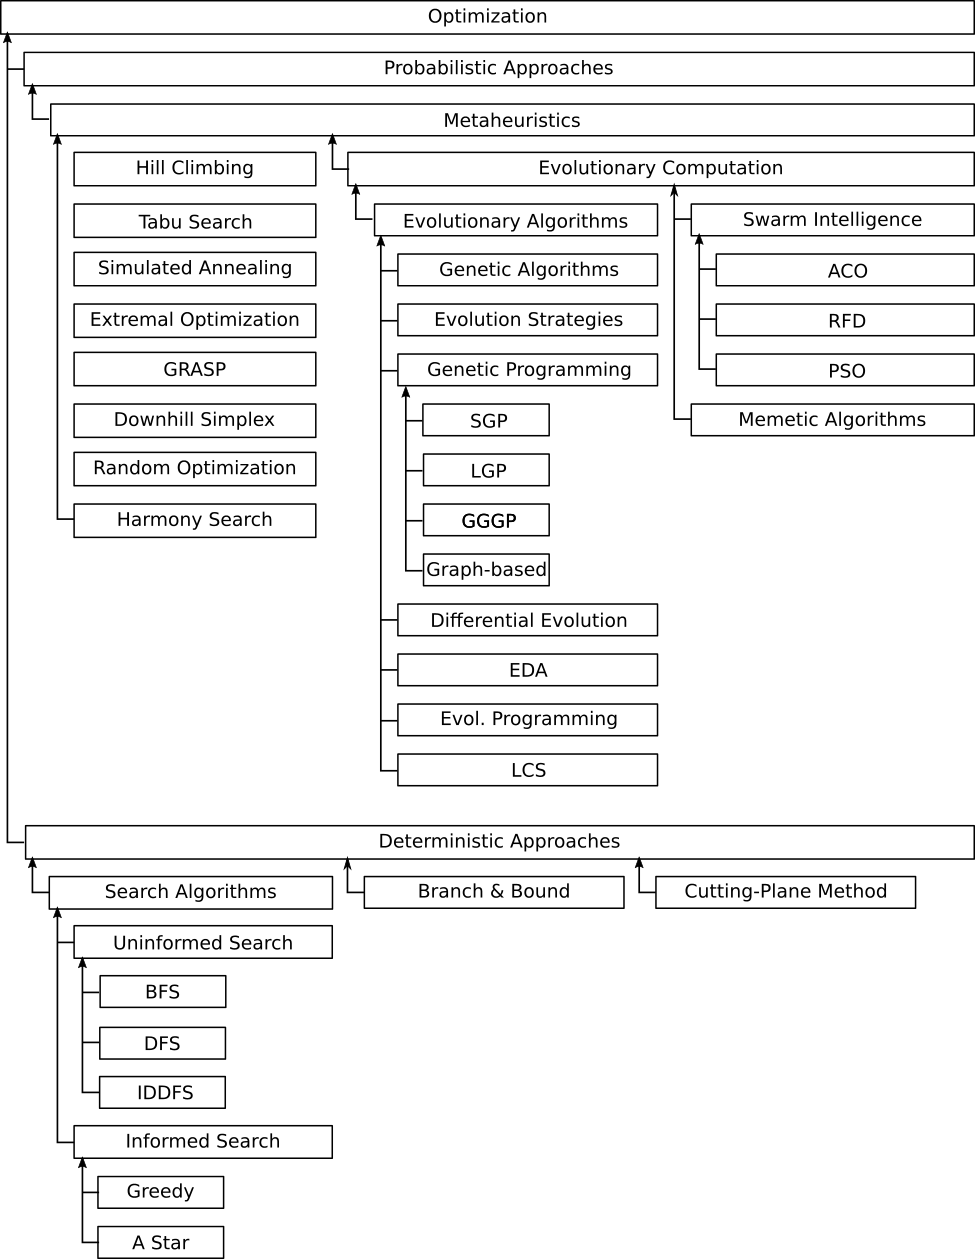
\includegraphics[width=.9\linewidth]{overview_optimisation_algorithm.png}
  \end{sidecaption}
\end{figure}

\subsection{Le domaine des algorithmes métaheuristiques, une sous-discipline de l'Optimisation}

\subsubsection{Q'est ce que l'optimisation ?}

Pour \textcite[22]{Weise2011}, l'optimisation \foreignquote{english}{ [...] is the process of solving an optimization problem, i. e., finding suitable solutions for it}, un problème d'optimisation nécessitant de trouver \foreignquote{english}{ [...] an input value $x^*$ for which a mathematical function $f$ takes on the smallest possible value (while usually obeying to some restrictions on the possible values of $x^*$ )}, la notation mathématique astérisque $^*$ désignant ici une valeur optimale.

Sortie de cette définition mathématique, l'optimisation peut également se définir par la mise en oeuvre d'algorithmes spécifiques. La littérature informatique met à disposition des programmeurs un ensemble d'algorithmes capables de fournir des solutions exactes dans un temps fini à un certain nombre de problèmes bien définis. C'est le cas par exemple des nombreux algorithmes de tri. Une autre classe d'algorithmes (\textit{optimization algorithms}) peut être employée lorsqu'il n'existe pas d'algorithme dédié (\textit{dedicated algorithms}), soit parce que le problème est trop spécifique, soit parce que personne n'a trouvé de solution efficace pour résoudre ce problème. 

Dans ce cadre, le terme d'optimisation globale \foreignquote{english}{ [...] is optimization with the goal of finding solutions $x^*$ for a given optimization problem which have the property that no other, better solutions exist.} Le terme \enquote{global} nécessite à la différence d'une recherche qui serait \enquote{locale}, de se concentrer sur l'obtention souvent plus couteuse et plus complexe d'un optimum global, minimum ou maximum, dominant par sa qualité l'ensemble des valeurs recherchées en entrée de la fonction à optimiser.

Bien que souvent beaucoup plus lent, moins précis, et plus consommateurs de ressources que les algorithmes du premier type, ces derniers nécessitent aussi beaucoup moins d'informations pour pouvoir être executés : \foreignquote{english}{Most often, these algorithms only need a definition of the structure of possible solutions and a function $f$ which tells measures the quality of a candidate solution. Based on this information, they try to find solutions for which $f$ takes on the best values.} \autocite[24]{Weise2011}

Ces algorithmes s'appuient donc sur différents types de stratégies pour tirer parti du peu d'information obtenue via cette fonction $f$. De nature très diverse, on retient pour séparer une première fois ces stratégies une typologie en deux classes. 

\begin{itemize}[label=\textbullet]
\litem{\textit{Probabilistic Approaches}} Les approches stochastiques désignées dans la fig. \ref{fig:S_OverviewOptimisation} sont capables de trouver un optimum assez rapidement, mais ne peuvent pas en garantir la propriété \enquote{globale}
\litem{\textit{Deterministic Approaches}} Les approches déterministes également désignées dans la fig. \ref{fig:S_OverviewOptimisation} peuvent certes garantir au moins théoriquement l'obtention d'un optimum global, mais s'éxecutent souvent au détriment d'un coût computationnel elevé.
\end{itemize}

Ces deux approches partagent également des difficultés communes, et découvrent leurs limites à des degrés divers en fonction des stratégies mise en oeuvre, dès lors que l'espace de recherche à parcourir devient trop important.

C'est le cas par exemple de l'espace de recherche de toute une sous-catégorie de problèmes \textit{NP-Complet} \Anote{np_complet_def} d'optimisation combinatoire \textit{Combinatorial Optimization Problems} (COP). Ce domaine contient par exemple les problèmes bien connus du voyageur de commerce \textit{Travelling salesman problem} (TSP), ou encore le problème du sac à dos \textit{Knapsack Problem} (KP) \Anote{note_knapsack}. Avec l'augmentation du nombre d'éléments entrant dans la définition de ces problèmes, il devient impossible de passer en revue l'ensemble des combinaisons (solutions possibles). Ce qui a pour conséquence de rendre difficile tout autant la découverte d'un optimum global, que la mesure de qualité de celui-ci, car pour établir cette dernière il nous faudrait logiquement connaitre la solution optimale, or c'est cela même que nous cherchons. 

Cette première typologie recoupe une autre propriété des algorithmes. La littérature informatique qualifie ainsi d'\textit{exacts} les algorithmes dont l'exécution garanti un résultat optimum à coup sûr, d'\textit{approximate algorithms} les algorithmes capables de donner une mesure proche d'un optimum sans pouvoir en garantir la qualité, et d'\textit{approximation algorithms} les algorithmes capables de donner une mesure proche d'un optimum assortie d'une preuve de qualité. Cette dernière classe n'est pas à confondre avec une classe d'algorithmes cherchant à conserver l'optimalité en limitant par diverses stratégies le coût temporel de résolution, mais bien l'inverse, relâcher la contrainte d'optimalité, mais aussi peu que possible. Les \textit{approximations algorithms} sont une donc une sous classe d'\textit{approximate algorithms}, et constituent une branche d'étude à eux seuls, car même dans le cas de problèmes \textit{NP-Complet}, ils offrent dans des dimensions raisonnables et propres à chacun des problèmes une solution sub-optimale d'erreur mesurable et donc potentiellement améliorable, voire comparable, notamment avec les résultats donnés de façon non analytique par d'autre stratégies.
%http://en.wikipedia.org/wiki/Approximation_algorithm#cite_ref-kann92onthe_3-4

On retrouve parfois rangé \enquote{en vrac} dans la classe des \textit{approximate algorithms} la classe des heuristiques et métaheuristiques - deux termes définis plus en détail dans la section suivante - mais cette typologie ne semble pas totalement juste non plus. 

Par exemple de multiples problèmes trouvent une solution exacte jusqu'à un certain niveau de complexification, à partir duquel on fait généralement appel aux heuristiques, soit par un appel à d'autres méthodes intégrant des heuristiques, soit par une intégration d'heuristiques aux méthodes existantes. Ainsi de nombreuses classes d'heuristiques sont utilisées de façon transversales, et apparaissent donc aussi comme composantes manipulées dans la classes des \textit{approximation algorithms}. L'heuristique gloutonne \textit{greedy algorithm} \Anote{greedy_description} apparaît de façon transversale à la fois comme une solution d'approximation pour le \textit{Knapsack Problem} (KP) mais également comme moteur dans le cadre d'algorithmes déterministes exacts comme la recherche du plus court chemin de Djikstra. Un autre algorithme nommé \textit{A*} (\textit{A-Star}) qui englobe Djikstra comme cas particulier, est quant à lui capable de fournir tout à la fois une mesure exacte ou approximée en fonction de l'heuristique injectée et du niveau de complexité du problème abordé. 

Dernier exemple, si les méthodes métaheuristiques sont effectivement souvent connues pour ne pas avancer de preuve, des travaux récents montrent toutefois qu'il existe de nouveaux algorithmes permettant de garantir dans certaines conditions un optimum global (CP-Algorithm de \autocite{Reuillon2014}). Tout dépend donc du degré et de la nature que l'on veut bien associer à la notion d'\textit{approximation} lorsqu'il s'agit de fournir une mesure d'éloignement de l'optimum. Les \textit{approximation algorithms} semblent toutefois plus intéressés par l'établissement d'une preuve au sens mathématique, et se concentrent avant tout sur un ensemble relativement limité de problèmes d'optimisation discret, ce qui ne semble pas être le but des métaheuristiques dans les deux cas. \autocite[1-6]{Kann1992} \autocite[13-15]{Williamson2011} %Metaheuristics: From Design to Implementation Par El-Ghazali Talbi

%You could think of a heuristic like an approximate (not approximation) solution to a problem. The difference between approximate and approximation is that the first is about getting a good guess of the solution of a problem, but that you don't really know how good it is. The second is about getting a solution for which you can prove how close it is to the optimal solution.

Enfin bien d'autres sous classifications sont possibles prenant plus ou moins en compte les spécificités propres aux différents algorithmes, comme celle opposant par exemple les stratégies utilisées en interne pour parcourir l'espace de recherche (generationel contre \textit{steady-state}, ou individuel contre populationel), la dimensionnalité possible pour la résolution des problèmes (mono-objectif contre multi-objectif), l'inspiration d'origine (naturelle biologique contre inspirations autres), etc. 

Toute classification monocritère est donc rendue très difficile, une voie s'étant même ouverte pour tenter de classer ces algorithmes suivant la nature et le niveau d'opération de ces hybridations. L'origine de cette difficulté tient dans une pratique courante et assumée d'hybridation entre les différentes techniques afin de réunir le meilleur de chacune d'elles au sein de nouvelle proposition de recherche. De fait, il est important pour la suite de cerner au mieux la classe d'algorithme d'optimisation que nous allons aborder, et de définir pourquoi nous l'avons abordé.

Nous nous intéresserons principalement dans la suite de cette présentation aux approches stochastiques métaheuristiques inspirées par la métaphore biologique, nommée \textit{Evolutionary Computation} (EC) ( voir figure \ref{fig:S_OverviewOptimisation}). La section \ref{xx} permettra de dégager les spécificités de cette subdivision, mais en attendant il nous faut d'abord présenter les principaux termes et concepts communs à tout les algorithmes d'optimisation. 

%On nomme métaheuristique (\textit{metaheuristic}) ce type d'algorithmes s'appuyant sur des heuristiques (\textit{heuristic}).

\subsubsection{Quelle définition peut on donner pour une heuristique (\textit{heuristic}) ? et une métaheuristique (\textit{metaheuristic}) ?}

Le terme heuristique \textit{heuristic} vient du Grec \textit{heuriskein} que l'on peut traduire par \foreignquote{english}{to find}, ou \foreignquote{english}{to discover}. D'usage plus large que dans la simple discipline informatique, nous retiendrons ici ce terme seulement sous son sens spécifique contextuel à l'optimisation. Rattaché à la définition d'un problème (\textit{problem dependent}), on définit une heuristique comme une mesure approximative pour définir la qualité d'une solution candidate \autocite[34]{Weise2011}.

%http://stackoverflow.com/questions/9140860/heuristic-function-for-finding-the-path-using-a-star
%http://stackoverflow.com/questions/9140860/heuristic-function-for-finding-the-path-using-a-star
%http://stackoverflow.com/questions/11779589/connection-between-a-star-search-and-integer-programming-extending-a-star
Si on se penche sur la classe d'algorithmes dédiés au problème de recherche du plus court chemin, les heuristiques sont souvent utilisées en appui des algorithmes de parcours de graphe, soit pour converger plus rapidement vers une solution optimale, soit pour justement se libérer de cette contrainte d'optimalité en visant un gain de temps au détriment de la précision. Si on prend par exemple l'algorithme de Djikstra, celui-ci n'utilise pas d'heuristique et garantit que le plus court chemin résultant sera optimal, car tous les chemins possibles entre le point de départ $A$ et le point final $B$ auront été analysés par celui-ci. Il est néanmoins connu comme étant très coûteux d'utilisation dès que le graphe dépasse un certain nombre de noeuds. L'algorithme déterministe $A^*$ s'appuie par contre sur une fonction heuristique $h(n)$ (une estimation du coût minimal reliant le noeud $n$ au noeud final) pour guider l'algorithme dans le processus incrémental de sélection d'un prochain noeud constitutif d'un chemin. En jouant sur cette heuristique, on est ainsi capable de déterminer si l'algorithme doit mettre la priorité sur la vitesse ou la précision, $h(0)$ étant équivalent ici à l'algorithme de Djikstra. Si l'heuristique est bien choisie (on dit ici que l'heuristique est admissible), alors $A^*$ garanti aussi l'optimalité du chemin trouvé, avec à la clef un coût computationnel moindre, car seule une partie des noeuds de l'ensemble du graphe auront été explorés par l'algorithme. Une autre heuristique misant plus sur la vitesse d'exécution pourra définir un chemin cette fois-ci sub-optimal avec un coût computationnel encore plus réduit. Il est à noter ici que l'utilisation d'une heuristique dans un programme n'est pas forcément motivée par la recherche d'un optimum global, mais par le gain de temps. Ainsi, un utilisateur peut très bien avoir les moyens d'obtenir un chemin optimal (Djikstra) sur une petite combinatoire de noeuds, mais peut vouloir prendre un raccourci en utilisant une méthode moins couteuse ($A^*$). Un scénario très souvent mis en avant dans la programmation de jeux sur ordinateur, où l'on cherche régulièrement à gagner du temps, tout en se rapprochant d'un comportement faillible imitant plus un adversaire de type humain.

Enfin, il faut noter que la forme prise par une heuristique est variable, et peut aller comme vu ci-dessus avec l'exemple $A^*$ d'une simple fonction mathématique de coût intégrée à un algorithme classique de parcours de graphes, à un algorithme beaucoup plus complexe intégrant de multiples prises de décisions pour estimer ce même coût. Dans le livre \textit{Code Complete} de \textcite[12]{McConnell2004}, celui-ci donne un exemple assez parlant pour illustrer la subtile différence qui sépare la description d'un algorithme employé au sens courant pour désigner un algorithme déterministe exact fournissant à coup sûr une solution, et la description d'un algorithme déterministe ou stochastique heuristique (ou appuyé par une heuristique) fournissant seulement un guide pour trouver, éventuellement, une solution.

\foreignquote{english}{Here's an algorithm for driving to someone's house: Take Highway's 167 south to Puyallup. Take the South Hill Mall exit and drive 4.5 miles up the hill. Turn right at the light by the grocery store, and then take the first left. Turn into the driveaway of the large tan house on the left, at 714 North Cedar}

\foreignquote{english}{Here's an heuristic for getting to someone's house: Find the last letter we mailed you. Drive to the town in the return adress. When you get to town, ask someone where our house is. Everyone knows us - someone will be glad to help you. If you can't find anyone, call us from a public phone, and we'll come get you.}

Le terme métaheuristique est lui aussi assez complexe à cerner. En effet pour \textcite{Luke2013} le terme métaheuristique est même en réalité plutôt malheureux pour définir cette catégorie d'algorithmes. Contrairement à ce que laisse entendre ce terme, \textit{une heuristique pour ou à propos d'une heuristique}, ce n'est donc pas de cela dont il s'agit ici.

Devant la difficulté de la tâche, et l'apparition de très nombreuses définitions, plusieurs auteurs semblent s'accorder pour faire du rattachement d'un algorithme à cette catégorie, une correspondance plus ou moins lâche avec un ensemble de propriétés généralement observées. En évitant une définition trop vague ou trop restrictive, on espère ainsi récupérer dans cette classe certains hybrides intéressants. 

Voici un exemple de propriétés issues de \textcite{Blum2003} et traduites ci dessous :

%label=$\blacktriangleright$
\begin{enumerate}[label=(\alph*),labelindent=\parindent,leftmargin=*]
	\item Les métaheuristiques sont des stratégies qui \enquote{guident} le processus de recherche. \label{enum_meta_a}
	\item Leur objectif est d'explorer l'espace de recherche efficacement pour trouver les solutions quasi-optimales. \label{enum_meta_b}
	\item L'étendues des techniques que constitue la classe des algorithmes métaheuristiques va de la simple recherche locale à un processus d'apprentissage complexe. \label{enum_meta_c}
	\item Les algorithmes métaheuristiques sont approximatifs et la plupart du temps non déterministes. \label{enum_meta_d}
	\item Les métaheuristiques peuvent incorporer des mécanismes pour éviter d'être piégé dans une portion confinée de l'espace de recherche. \label{enum_meta_e}
	\item Les concepts de bases des métaheuristiques permettent d'adopter un certain degré d'abstraction dans la description. \label{enum_meta_f}
	\item Les métaheuristiques ne sont pas \textit{problem-specific}. \label{enum_meta_g}
	\item Les métaheuristiques peuvent faire usage d'une expertise du domaine au travers des heuristiques controlées par une stratégie de plus haut niveau. \label{enum_meta_h}
	\item La plupart des métaheuristiques actuelles font appel à une mémoire pour améliorer le processus qui guide la recherche. \label{enum_meta_i}
\end{enumerate}

Afin de mieux comprendre cette table de propriétés un peu abstraite, il est proposé de reprendre ces différents points au travers d'une lecture commentée.

Le terme métaheuristique est d'origine plus moderne (1986), et a permis d'englober a posteriori des algorithmes jusque là qualifiés d'heuristiques. C'est le cas par exemple d'une bonne partie des algorithmes évolutionnaires, qui émergent principalement au cours des années 1960-1970. 

Voici comment \textcite[8]{Brownlee2012} perçoit la différence entre les deux termes : \foreignquote{english}{Like heuristics, metaheuristics may be considered a general algorithmic framework that can be applied to different optimization problems with relative few modifications to adapt them to a specific problem. The difference is that metaheuristics are intended to extend the capabilities of heuristics by combining one or more heuristic methods (referred to as procedures) using a higher-level strategy (hence ‘meta’). A procedure in a metaheuristic is considered black-box in that little (if any) prior knowledge is known about it by the metaheuristic, and as such it may be replaced with a different procedure. Procedures may be as simple as the manipulation of a representation, or as complex as another complete metaheuristic. Some examples of metaheuristics include iterated local search, tabu search, the genetic algorithm, ant colony optimization, and simulated annealing.}

Le terme \enquote{méta-} renvoie plus en définitive au concept générique de \enquote{stratégie de recherche} prenant la forme d'un algorithme d'optimisation capable de mélanger, manipuler des heuristiques ou d'autres métaheuristiques (cf. points \ref{enum_meta_a} et \ref{enum_meta_h}) \Anote{def_meta_weise}. Contrairement aux heuristiques, les métaheuristiques se définissent plus comme un système fait de composants, dont la plasticité permet le support et l'interaction nécessaire au développement d'heuristiques plus ciblées (\textit{problem dependent}) \Anote{def_meta_sorensen}. La structure offre un patron d'usage initial (\textit{pattern}) qui reste indépendant du problème abordé (\textit{problem independent}) (cf. \ref{enum_meta_g}), tout en restant évolutif, comme le montre le fort développement de cette discipline depuis les années 1980. Ce principe de flexibilité, on le retrouve par exemple dans la classe des EC, comme le mettent bien en valeur Bach, Hammel et Schwefel en 1997, dans une publication introduisant l'EC dans la série renommée des \textit{IEEE Transactions} :

\foreignquote{english}{We argue that the most signicant advantage of using evolutionary search lies in the gain of exibility and adaptability to the task at hand, in combination with robust performance (although this depends on the problem class) and global search characteristics. In fact, evolutionary computation should be understood as a general adaptable concept for problem solving, especially well suited for solving difficult optimization problems, rather than a collection of related and ready-to-use algorithms. The majority of current implementations of evolutionary algorithms descend from three strongly related but independently developed approaches: genetic algorithms,evolutionary programming , and evolution strategies. [...] The fundamental difference in the evolutionary computation approach is to adapt the method to the problem at hand. In our opinion, evolutionary algorithms should not be considered as off-the-peg, ready-to-use algorithms but rather as a general concept which can be tailored to most of the real-world applications that often are beyond solution by means of traditional methods. Once a successful EC-framework has been developed it can be incrementally adapted to the problem under consideration, to changes of the requirements of the project, to modifications of the model and to the change of hardware resources.} \autocite{Back1997a}

\hl{transition}

\textit{Comment se matérialise la recherche de solutions optimisées dans une métaheuristique ?}

Contrairement à d'autres méthodes d'optimisations, les métaheuristiques font généralement appel à un processus d'échantillonnage \ref{enum_meta_b} pour explorer de façon stochastique un espace de recherche de toute façon beaucoup trop vaste pour être parcouru de façon exhaustive.

C'est pour cela que \textcite[7]{Luke2013} nous propose de voir ce type de problème autrement, partant du postulat assez logique qu'une solution \enquote{même non optimale} est un point de départ pour l'amélioration de toute façon bien meilleure que \enquote{pas de solution du tout}.

\foreignquote{english}{ Metaheuristics are applied to \enquote{I know it when I see it} problems. They're algorithms used to find answers to problems when you have very little to help you: you don't know what the optimal solution looks like, you don't know how to go about findint it in a principled way, you have very little heuristic information to go on, and brute-force search is out of the question because the space is too large. But if you're given a candidate solution to your problem, you can test it and assess how good it is. That is, you know a good one when you see it.}  

\hl{schéma}

Suivant ce raisonnement, la connaissance d'un problème se construit au travers d'une confrontation répétée de nos représentations, de nos interrogations avec la forme réelle et encore inconnue prise par celui-ci. La carte de ce nouveau territoire se révélant peu à peu dans la projection sur l'espace des solutions des choix effectués lors de la sélection des nouveaux candidats à évaluer (solutions candidates).

Les métaheuristiques sont donc là pour faciliter l'exécution de cette tâche complexe et répétitive qui consisterait à améliorer notre connaissance du problème en proposant de façon pertinente de nouvelles solutions candidates à évaluer, ces dernières étant choisies si possible en fonction des résultats obtenus par les précédentes (voir point \ref{enum_meta_i}). La perspective d'une telle automatisation pose évidemment un certain nombre de questions. 

Quels sont les choix mis à disposition de l'optimiseur pour améliorer la réponse attendue des solutions candidates entre chaque incrément ? \autocite[19]{Weise2011} 

Une comparaison automatisée nécessite pour être mise en oeuvre de définir \begin{enumerate*}[label=(\alph*)]
\item sur quelle base se fonde l'évaluation d'une solution,
\item la comparaison entre les solutions évaluées, 
\item et la sélection de nouvelles solutions candidates.\end{enumerate*} Car l'optimiseur, tout comme nous, ne connait pas directement la forme prise par l'espace des solutions, et doit bien concevoir en interne les choix permettant, par la selection de nouvelles solutions candidates à évaluer, de progresser si possible vers une solution optimum.

De fait dans un tel scénario, et pour éviter une recherche aléatoire, l'évaluation de solution candidate renvoie à l'existence d'une expertise externe à l'optimiseur, le seul capable de formaliser ce qui différencie une bonne solution d'une mauvaise solution. On revient à parler ici d'heuristique, et de leurs diversités, car si celles-ci interviennent dans l'évaluation des solutions candidates (a), elles interviennent aussi dans les autres cas (b) et (c). Elles se présentent sous la forme de différents types de connaissances, interrogent différents espaces, et s'intègrent souvent sous la forme de composants dans la structure plastique des métaheuristiques.

L'injection de connaissance (voir point \ref{enum_meta_h} )dans ce type d'algorithme métaheuristique est donc double, et opère à la fois de façon précise dans la formalisation d'un ou de plusieurs critères qui vont servir pour l'algorithme optimiseur à déterminer la qualité, bonne ou mauvaise, d'une solution candidate; et de l'autre elle intervient cette fois ci de façon moins contrôlable dans la façon dont l'expérimentateur va construire et paramétrer une métaheuristique pour l'adapter au mieux à son problème. La qualité interne (paramètre, structure) de la métaheuristique définit aussi en quelque sorte le processus d'exploration, ce qui explique aussi la dépendance de ce type d'algorithmes à l'environnement qu'ils doivent explorer.

\begin{figure}[ht]
	\begin{sidecaption}[fortoc]{Projection du vecteur de points $\{a \dotsc n\}$ dans l'espace des objectifs. Les couleurs représentent les différents axes de projection ordonnés de 1 à 3 sur $(x,v)$ et de 1 à 4 sur $(y,v)$}[fig:spacePspaceOmultimodal]
	 \centering
	 	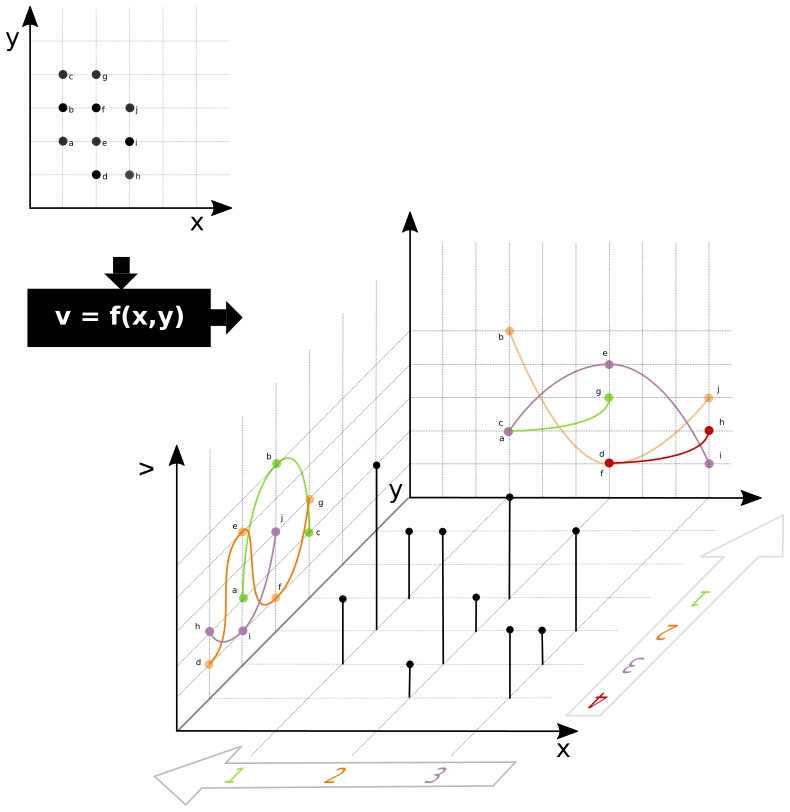
\includegraphics[width=.9\linewidth]{espaceP_espaceO_multimodal.pdf}
	\end{sidecaption}
\end{figure}

L'objectif est rendu complexe car la relation entretenue entre ces deux espaces, celui des solutions candidates disponibles, et celui des évaluations est bien souvent dissymétrique. Pour mieux comprendre cette relation, la figure \ref{fig:spacePspaceOmultimodal} illustre cette correspondance des solutions candidates $\{a \dotsc n\}$ décrites par leurs coordonnées $(x,y)$ lorsqu'elles sont projetées dans l'espace des objectifs $\mathbb{Y}$ en suivant la transformation attendue par la fonction boite noire de dynamique non linéaire $f(x,y)$. Les valeurs $v = f(x,y)$ des différentes solutions candidates sont également projetées sur le plan 2D $(x,v)$ et $(y,v)$ pour mieux visualiser la forme prise par cette surface en 2D.

\begin{figure}[!htbp]
	\begin{sidecaption}[fortoc]{Les couleurs indiquent la  des valeurs $v = f(x,y)$ mesurée dans la figure \ref{fig:spacePspaceOmultimodal}, sachant qu'on cherche à minimiser la valeur de v :
\parbox{\marginparwidth}{
\begin{enumerate}[label={},labelindent=0pt,leftmargin=*]
        \item \sqbox{tangoBlue1} indique une fitness minimale, cf. qui maximise $v$
        \item \sqbox{tangoOrange1} indique une fitness intermédiaire et,
        \item \sqbox{tangoRed1} indique une fitness maximale, cf. qui minimise $v$
\end{enumerate}}}[fig:xyspacePspaceOmultimodal]
	 \centering
	  \subbottom[]{
	 	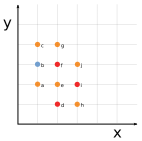
\includegraphics[width=0.4\linewidth]{xyespaceSolutionCandidate_a.pdf}
	 	\label{subfig_xyespaceSolutionCandidate_a}}
	 \subbottom[]{
	 	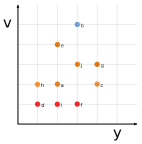
\includegraphics[width=.4\linewidth]{xyespaceSolutionCandidate_b.pdf}
	 	\label{subfig_xyespaceSolutionCandidate_b}}
	 \subbottom[]{
		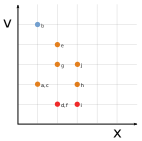
\includegraphics[width=.4\linewidth]{xyespaceSolutionCandidate_c.pdf}
		\label{subfig_xyespaceSolutionCandidate_c}}
	\end{sidecaption}
\end{figure}

Pour visualiser la valeur $v$ prise par chacune des solutions candidates, on projette celle-ci dans l'espace $(x,y)$, ce qui nous permet de mieux constater l'éclatement des valeurs de $v$ sur la figure \ref{fig:xyspacePspaceOmultimodal}.

Deux solutions proches dans l'espace des solutions candidates peuvent amener à des résultats très différents, et inversement, pour deux évaluations proches peuvent correspondre des solutions candidates très éloignées, comme le détaille la figure \ref{fig:xytrajectoire}. Il s'agit d'une propriété bien connu des fonctions non linéaires, qu'elles soient décrites de façon explicite via le formalisme mathématique, ou de façon implicite dans l'expression des dynamiques complexes de modèles de simulation.

Il est clair que l'information récoltée par un tel déplacement basé sur une distance euclidienne dans le plan $(x,y)$ n'est pas vraiment pourvoyeur d'intuitions sur l'emplacement possible des meilleures solutions (voir figure \ref{fig:xytrajectoire}). Il semble par exemple plus intéressant pour l'optimiseur d'accéder aux solutions par le prisme d'ensembles construits sur la base d'une valeur $v$ commune (voir figure \ref{fig:xyspacePspaceOmultimodal}). Une information qui peut être exploitée de multiples façons, toujours en permettant à l'optimiseur de déterminer un nouvel ensemble de solutions candidates à évaluer.

\begin{figure}[!htbp]
	\begin{sidecaption}[fortoc]{Représentation de deux déplacements dans l'espace des solutions candidates et son équivalent dans l'espace des objectifs
	\parbox{\marginparwidth}{
	\begin{enumerate}[label=(\alph*),labelindent=\parindent,leftmargin=*]
	        \item Partant de $b$, on se déplace d'une unité vers $c$ ou $a$, ce qui dans l'espace des objectifs équivaut également à un déplacement vers $h$; $v=2$ pour $v_h, v_a, v_c$
	        \item Partant de $b$, on se déplace toujours d'une unité vers $f$, ce qui dans l'espace des objectifs équivaut également à un déplacement vers $d$ et $i$; $v=1$ pour $v_d,v_i,v_f$
	\end{enumerate}}}[fig:xytrajectoire]
	 \centering
	  \subbottom[]{
	 	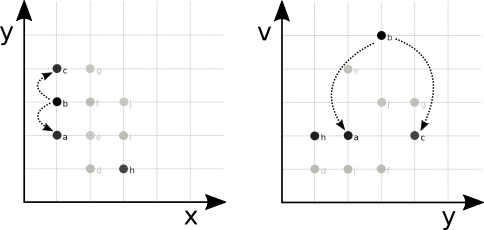
\includegraphics[width=0.6\linewidth]{xytrajectoire_a.pdf}
	 	\label{subfig_xytrajectoire_a}}\qquad
	 \subbottom[]{
	 	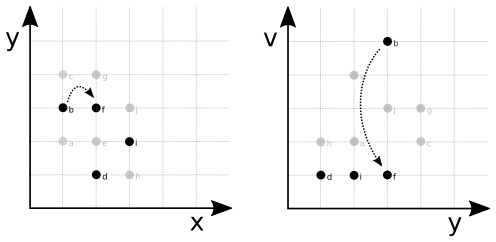
\includegraphics[width=.6\linewidth]{xytrajectoire_b.pdf}
	 	\label{subfig_xytrajectoire_b}}
	\end{sidecaption}
\end{figure}

Si l'obtention d'une cartographie complète d'un tel espace de solutions peut être l'objectif de ce type de raisonnement, la recherche d'un optimum en est un autre. Dans un cas on aura tendance à maximiser la diversité dans le choix de solutions candidates à évaluer, afin d'essayer de couvrir au mieux le territoire à explorer. Cette idée on la retrouve dans l'établissement d'une \textit{fitness landscape}, ou dans sa version multi-objectif, d'un \textit{problem landscape} \autocite[93-94]{Weise2011}, un paysage cumulé de l'espace des objectifs indiquant toutes les valeurs prises par ceux-ci au cours de l'exploration \Anote{paysage_cumule}. Un espace mis à profit par l'optimiseur pour améliorer la proposition de solution candidate, par exemple en se basant sur la construction de cluster de valeurs intéressantes comme indiqué précédemment, ou encore en cherchant à favoriser les zones de cet espace encore peu explorées, etc. Alors que dans le cas d'une optimisation pour la calibration ou la prédiction, trouver le plus rapidement possible un minimum local ou global peut constituer un objectif suffisant.

En réalité, ces deux objectifs sont souvent liés, et c'est souvent l'expertise humaine intervenant de façon externe à l'optimiseur qui va déterminer l'importance de l'un ou de l'autre dans la stratégie à suivre. Dans le cas par exemple d'une optimisation de paramètres nécessaire à la marche efficiente d'une centrale nucléaire, la découverte d'un minimum local robuste peut s'avérer beaucoup plus intéressante qu'un minimum global instable. La topologie proche de l'espace des solutions déjà exploré peut constituer un facteur de connaissance d'intervention plus ou moins importante dans l'expertise d'une bonne ou d'une mauvaise solution. 

Cette mécanique on la retrouve également à un autre niveau, dans le fonctionnement interne des métaheuristiques. En effet, celles-ci s'appuient le plus souvent sur la métaphore biologique évolutive pour mettre en tension une recherche de solutions guidée toute à la fois par l'\textit{exploration} (trouver des solutions originales), et l'\textit{exploitation} (améliorer les solutions existantes). 

\begin{figure}[!htbp]
\begin{sidecaption}[fortoc]{Recherche d'un minimum global.}[fig:hmap2ab]
 \centering
 \subbottom[Une fonction $f(x)$ présentant un unique minimum global]{
 	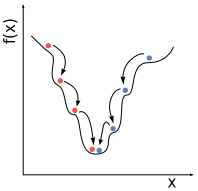
\includegraphics[width=.4\linewidth]{heightmap2a.pdf}
 	\label{subfig_hmap2ab_a}}\qquad
 \subbottom[Une fonction $f(x)$ présentant un minimum local et global]{
	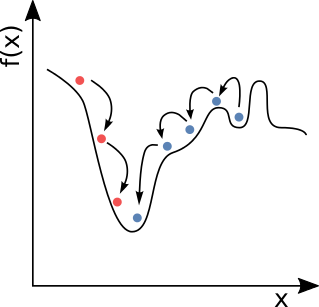
\includegraphics[width=.4\linewidth]{heightmap2b.pdf}
	\label{subfig_hmap2ab_b}}
\end{sidecaption}
\end{figure}

Les opérateurs intervenant comme stratégies dans la médiation de ces deux concepts sont conçus pour éviter à l'optimiseur un certain nombre d'écueils. Trop longue pour être abordée ici de façon exhaustive, cette liste évoquant les problèmes et solutions qui résultent du rapport entre les formes de problèmes abordés et les faiblesses génériques ou dépendantes des métaheuristiques utilisées, \textcite{Weise2011} en donne une description experte sur une centaine de pages. On peut également se référer à une autre synthèse, abordant ces problèmes avec un angle un peu plus spécifique aux algorithmes évolutionnaires, réalisée en 2001 par \textcite[316-445]{Deb2001}.

En se limitant aux pièges dépendant de la topologie de l'espace des solutions (voir point \ref{enum_meta_e}), \textcite[140]{Weise2011} a proposé un tableau synthétique dont on extrait ici quelques exemples légèrement modifiés pour éclairer notre argumentaire. Les exemples des figures \ref{fig:hmap2ab} et \ref{fig:hmap2cd} mettent en oeuvre un optimiseur générant de façon incrémentale de nouvelles solutions, chacune représentée par un point. Il faut donc visualiser ces exemples en tenant compte du fait qu'ils présentent une représentation cumulative des différents points parcourus dans le temps par l'optimiseur.

La figure \ref{fig:hmap2ab} démontre un fonctionnement normal de l'optimiseur, capable quelque soit son placement initial (rouge ou bleu), de trouver le minimum global d'une fonction relativement simple \ref{subfig_hmap2ab_a}. Un comportement équivalent est observable dans la figure \ref{subfig_hmap2ab_b}, le compromis \enquote{exploitation - exploration} étant suffisant pour que l'optimiseur bleu surmonte l'obstacle posé par la présence d'un minimum local dans cette fonction.

\begin{figure}[!htbp]
  \begin{sidecaption}[fortoc]{Deux types de fonctions sont rendues difficiles à optimiser du fait d'une topologie marquée.}[fig:hmap2cd]
  \centering
  \subbottom[Une fonction $f(x)$ multimodale acceptant plusieurs minimum locaux, et un seul minimum global]{
  	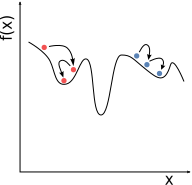
\includegraphics[width=.4\linewidth]{heightmap2e.pdf}
  	\label{subfig_hmap2cd_c}}\qquad
  \subbottom[Une fonction $f(x)$ contenant très peu d'information de gradient pour guider l'optimiseur]{
	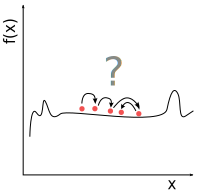
\includegraphics[width=.4\linewidth]{heightmap2c.pdf}
  	\label{subfig_hmap2cd_d}}
 \end{sidecaption}
\end{figure}

A l'inverse, on perçoit bien sur ce schéma \ref{subfig_hmap2cd_c} quel effet peut avoir un déséquilibre entre les deux stratégies, une exploitation trop appuyée au détriment de l'exploration amenant souvent à une convergence \Anote{def_convergence} prématurée, c'est-à-dire à un piège dans un optimum local. 

La figure \ref{subfig_hmap2cd_d} montre également que face à une topologie de fonction présentant un plateau relativement uniforme, l'optimiseur sera en peine pour trouver un minimum, même local. Un paramétrage différent de l'exploration pourra peut être résoudre ce problème, sans pour autant que l'on en soit sur. 

Ce qui nous permet d'évoquer une faiblesse connue des métaheuristiques, héritée des remarques déjà faites sur les algorithmes d'optimisations stochastique \Anote{stochastic_note} dans laquelle on les place habituellement. La découverte garantie d'une solution globale optimale est en général difficile avec ce type d'algorithmes (voir point \ref{enum_meta_d}) \Anote{equipe_mixite}, au moins pour deux raisons : 

\begin{enumerate}
\item la variabilité qui opère lors de la selection des solutions candidates à un instant $t$ ne permet pas de garantir qu'il n'existe pas quelque part une solutions candidate selectionné à $t+1$ dont l'évaluation révélera un meilleur optimum. La définition d'un critère d'arrêt est donc rendu délicate.
\item La variabilité dans l'établissement d'une trajectoire de recherche implique qu'un algorithme de même qualité puisse passer une première fois à coté d'un optimum, et une deuxième fois trouver celui-ci. 
\end{enumerate}

\begin{figure}[!htbp]
\begin{sidecaption}[fortoc]{Représentation d'une navigation indirecte de l'optimiseur dans un espace de solution $z = f(x,y)$.}[fig:hmap1]
  \centering
  \subbottom[]{
  	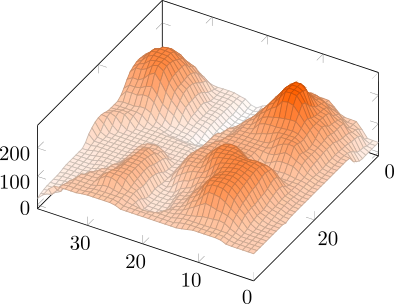
\includegraphics[width=.4\linewidth]{heightmap1a.png}
  	\label{subfig_hmap_a}}\qquad
  \subbottom[]{
	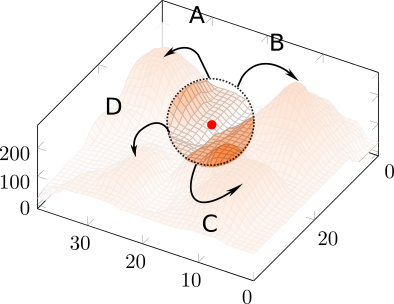
\includegraphics[width=.4\linewidth]{heightmap1b.png}
  	\label{subfig_hmap_b}}
\end{sidecaption}
\end{figure}

Pour mieux comprendre les problèmes posés par des espaces de solutions multi-modaux, déjà figurés en deux dimensions dans \ref{subfig_hmap2cd_c}, on représente cette fois ci dans la figure \ref{fig:hmap1} l'optimiseur dans un espace en trois dimensions similaire à celui vu dans la figure \ref{fig:spacePspaceOmultimodal}, à la recherche d'un optimum global. La fonction ainsi représentée comporte deux entrées $(x,y)$, et une sortie $z = f(x,y)$ représentant la valeur numérique résultat de l'optimisation.

Attention à la lecture de ces schémas, il ne faut pas oublier que l'optimiseur \textbf{ne se déplace pas directement} sur le terrain visible dans la figure \ref{subfig_hmap_a}, et pour laquelle celui-ci n'a justement aucune visibilité. C'est un peu comme visualiser un labyrinthe de l'extérieur sur une feuille, puis de l'intérieur quand on s'y projette, la difficulté pour résoudre celui-ci n'est plus la même. La visibilité dont dispose l'optimiseur est celle des résultats de solutions candidates déjà évaluées (voir point \ref{enum_meta_i}). Il s'agit donc de proposer de nouvelles solutions candidates soit en les composant à partir d'une manipulation des solutions candidates déjà évaluées, soit en introduisant de toutes nouvelles solutions candidates prises de façon aléatoire. Au cours de l'itération mesurant la progression de l'algorithme, c'est bien l'évaluation de cette nouvelles population de solutions candidates qui détermine si il y'a effectivement eu un déplacement qualitatif dans l'espace des solutions evaluées. Le déplacement du point rouge dans cet espace n'est donc effectif que si on trouve à un instant $t + 1$ une solution plus intéressante qu'à l'instant $t$.

A partir des résultats de la première solution candidate évaluée figurée ici en rouge dans \ref{fig:hmap1}, les opérateurs de recherches soumis à l'aléa d'une recomposition ou d'un tirage aléatoire peuvent tout à fait proposer un candidat à $(x,y)_{t+1}$ qui débouche sur un résultat $z = f(x,y)$ plaçant l'optimiseur dans le sillon d'un gradient de pente parmi plusieurs. Ce qui mènera probablement l'optimiseur à découvrir des optimums de qualités très différentes : $A$ (local), $B$ (global), $C$ (local), $D$ (local). 

Autrement dit, en plus de la stochasticité inhérente de ces algorithmes, non seulement un algorithme de type $A$ n'aura pas les mêmes résultats qu'un algorithme de type $B$, mais celui-ci sera également différent d'un algorithme $A'$ du fait d'un paramétrage différent.

Comme déjà évoqué dans les différentes définitions, on retrouve ici la qualité de flexibilité des métaheuristiques, permettant de transformer ce qui pourrait de prime abord paraitre pour un défaut, en qualité. L'utilisation de celle-ci permettant d'étendre toujours un peu plus leurs champs d'utilisation, en facilitant la réponse aux questions suivantes \Anote{q_ppr} : 
\begin{enumerate}
\item  \foreignquote{english}{What parameter settings do I use to get good results when applying heuristic method X to problem Y?}
\item  \foreignquote{english}{How do I adjust the parameters of heuristic X so I get better results on problem Y?}
\item \foreignquote{english}{Which is \enquote{better}, heuristic X or heuristic Y?}
\end{enumerate}

On pourrait ainsi ne retenir que cette citation de source inconnue, lorsqu'elle définit une métaheuristique comme \foreignquote{english}{ a pretty good rule for finding pretty good rules.}

Cette flexibilité vient compléter et compenser efficacement cet horizon de connaissance assez limité, nécessaire à une généricité d'emploi. Les métaheuristiques fournissent ainsi le support générique initial pour en faire un outil d'usage indépendant du problème, tout en fournissant les outils pour favoriser également leur propre modification en vue d'une amélioration de résultat pour un problème donné. Elle cumule donc en quelques sortes les deux propriétés de dépendance et d'indépendance face à un problème donné. 

De plus, la recherche dans cette discipline ne se contente pas d'organiser une forme de compétition qui mènerait à elle seule, par l'apprentissage répété de fonctions aussi standardisées que celles utilisées dans les figures précédentes, à une surestimation de certains algorithmes \Anote{test_fonction_surutilisation}, et se nourrit également d'une recherche plus appliquée à des problématiques réelles. Ce qui permet par effet retour, d'espérer voir appliquer à des formes de problèmes génériques, des opérateurs dédiés à l'origine à des problématiques spécifiques. La construction et l'évaluation d'heuristique plus performante servant toujours indirectement une cause plus générale.

Enfin, une des propriétés qui n'a pas encore été introduite dans ce résumé est la capacité de notation et de description abstraite des métaheuristiques (voir point \ref{enum_meta_f} ). Des concepts de plus haut niveau sont introduits pour désigner l'expression et la manipulation d'heuristiques et de classes d'heuristiques dans un système composant la métaheuristique. Mais avant de pouvoir introduire ces subtilités de typologie propre à chaque classe de métaheuristique, il faut également rappeler l'existence d'une base commune de formalisation mathématique permettant la description des problèmes. Autrement dit, cela revient à introduire ou à poser sur une partie des mots déjà utilisés dans cette section, un certain nombre de notations mathématiques d'utilisation relativement standard dans cette communauté informatique utilisant les métaheuristiques.

Il nous restera également à aborder dans la section suivante, la question des \textbf{moyens} mis à disposition de l'optimiseur pour opérer la selection de nouveaux candidats à évaluer. Jusqu'ici seule une représentation de ces solutions candidates dans l'espace des solutions candidates possibles a été abordée, ainsi que l'espace contenant les résultats des solutions candidates évaluées. Mais ces deux espaces ne constituent pas les véritables espaces sur lesquels l'optimiseur est amené à travailler, et cela bien qu'il puisse les intégrer à son expertise pour la selection de nouveaux candidats à l'évaluation \Anote{remarque_section_metaheuristique}. 

\hl{les 4 paragraphe ci dessous sont à faire descendre avec notation mathématique, pour compléter la section suivante, et sans briser le suspens ?}

L'introduction d'un nouvel \enquote{espace de recherche} est nécessaire, et  correspond à la somme des entrées, des paramètres, sur lequel l'optimiseur va pouvoir jouer directement, afin de modifier cette fois-ci indirectement l'expression de la solution candidate ensuite évaluée.

Autrement dit, il faut retenir qu'une solution candidate fait partie d'un espace de solutions candidates possibles, et que l'exploration de ce dernier est dépendant des bornes fixés par l'expert pour délimiter l'espace de recherche de chacun des entrant, notamment pour limiter le champ de recherche de l'optimiseur à celui des valeurs empiriquement et théoriquement possibles. Ce qui introduit aussi la possibilité d'une nouveau \textit{mapping} entre les valeurs de ces deux espaces, de recherche, et du phénomène à évaluer, qui ne sont pas nécessairement de même nature. 

On peut s'appuyer sur l'exemple de bras robotisé donné par \autocite{Weise2011} pour illustrer ce cas. On a d'un côté les paramètres de positionnement des éléments de bras d'un robot, contraint par la structure théorique de celui-ci, et de l'autre l'expression spatiale finale du bras représentatif de cette combinaison de paramètres dans l'espace des solutions possibles, potentiellement infini, et dont on n'a pas la maitrise directe. L'optimiseur s'appuie ensuite sur l'évaluation de cette configuration spatiale à l'aide des critères qu'on lui a donné pour induire des opérations non pas dans l'espace d'expression spatialisé du bras, mais dans l'espace de recherche des vecteurs de paramètres permettant l'amélioration de ce résultat.

\subsubsection{Une formulation mathématique standardisée pour encadrer les problème d'optimisation et les métaheuristique}

%search space p 82
%structure p 101
% pareto ranking p 275
																								
Pour comprendre comment se déroule de façon générale la résolution d'un problème d'optimisation, il faut poser un certain nombre de notions qui nous seront utiles par la suite. Cet exercice de description plus mathématique et générique s'appuie là encore principalement sur les écrits de \textcite{Weise2011}

La première étape selon Weise dans la construction d'un problème d'optimisation est de définir le type de structure qui peut être associée à l'expression des solutions possibles et spécifiques à notre problème.

Autrement dit, il s'agit de déterminer quel est l'espace dans lequel évolue la donnée figurant la solution attendue pour cette optimisation. L'expression de cette solution peut appartenir à l'espace des réels $\mathbb{R}$, comme par exemple une valeur numérique se rapportant à l'optimisation d'une fonction mathématique. Mais celle-ci peut également s'exprimer dans un repère beaucoup plus complexe, en faisant référence par exemple à un repère géométrique définissant le cadre  d'une forme à optimiser comme une pièce de moteur, une pièce d'avion, etc. \autocite[43]{Weise2011}

Cet espace du problème (\textit{problem space}) $\mathbb{X}$ est défini comme \foreignquote{english}{ [...] the set containing all elements $x$ which could be its solution.} 

Une solution candidate $x$ est quant à elle définie comme \foreignquote{english}{ [...] an element of the problem space $ \mathbb{X}$ of a certain optimization problem.}

L'objectif de l'optimisation est donc de trouver par le biais d'un algorithme adapté l'ensemble des solutions candidates $x^*$ appartenant à l'espace du problème répondant le mieux aux critères définis par l'utilisateur. Ce qui suppose de pouvoir qualifier une solution candidate $x_1$ tiré de $\mathbb{X}$ par rapport à une autre solution candidate $x_2$ elle aussi tiré de $\mathbb{X}$.

\textit{Une deuxième étape logique serait donc d'établir comment se fait la mesure établissant la qualité d'une solution ?}

Comme défini précédemment, ce qui va guider l'algorithme optimiseur dans sa prise de décision, c'est l'évaluation d'une fonction heuristique, ou d'une fonction objectif (\textit{objective function}) \Anote{difference_objective_heuristique} 

\foreignquote{english}{An objective function $f: \mathbb{X} \mapsto \mathbb{R}$ is a mathematical function which is subject to optimization.}

Cette fonction objectif lorsqu'elle prend pour paramètre un élément candidat $x$ pris dans l'espace du problème $ \mathbb{X}$ renvoie une valeur définissant sa qualité par rapport au problème posé. \autocite[44]{Weise2011}

\sloppy La plupart des problèmes nécessitent toutefois d'optimiser plusieurs critères simultanément. La relation entre ces critères peut d'ailleurs être elle aussi multiple : dépendante (conflictuelle, en harmonie), indépendante. Nous allons donc nous intéresser directement à la définition de ce type de problème, résumable ainsi :  $min(f_1(x), \dotsc, f_k(x)$ avec $k > 2$

La littérature fait également plus souvent référence à ce type de problème en faisant appel à une notation sous forme de fonction vecteurs. Un ensemble $\vec{f} : \mathbb{X} \mapsto \mathbb{R}^n$ fait de $n$ fonction objectif $f_i : \mathbb{X} \mapsto \mathbb{R}$ avec $\forall i \in 1 \dotsc n$. Appliqué à une solution candidate $x \in \mathbb{X}$ cette fonction renvoie un vecteur de réel de dimension $n$ qui peuvent être projeté dans un espace $\mathbb{R}^n$, aussi appelé espace des objectifs (\textit{objective space}) $\mathbb{Y}$.

En résumé, à chaque association d'un vecteur de fonction objectif $\vec{f}$ et d'une solution candidate $x$ correspond après évaluation un vecteur de réel de dimension $n$ permettant le positionnement de la solution candidate dans l'espace $\mathbb{R}^n$ des objectifs aussi nommé $\mathbb{Y}$.

C'est à partir du positionnement des solutions candidates dans cet espace $\mathbb{Y}$ que l'optimiseur va décider de la prochaine solution candidate à évaluer. 

\textit{Dès lors, comment ce choix se fait-il dans une perspective multi-objectif a priori contradictoire ?}

\begin{figure}[!hbtp]
	\begin{sidecaption}[fortoc]{ Pour la valeur $x = 0$, $f1(x) = 0 $ et $f2(x) = 4 $, pour $x = 2$,  $f1(x) = 4 $ et $f2(x) = 0 $ , donc la configuration inverse. La solution pour minimiser les deux fonctions $f1$ et $f2$ tient donc forcément dans un compromis dans la valeur prise par $x$.}[fig:S_Schaffer]
	\centering
	\begin{tikzpicture}[line cap=round,line join=round,>=triangle 45,x=1.0cm,y=1.0cm]
	\draw [color=cqcqcq,dash pattern=on 1pt off 1pt, xstep=1.0cm,ystep=1.0cm] (-5,-1) grid (5,5);
	\draw[->,color=black] (-5,0) -- (5,0);
	\foreach \x in {-5,-4,-3,-2,-1,1,2,3,4}
	\draw[shift={(\x,0)},color=black] (0pt,2pt) -- (0pt,-2pt) node[below] {\footnotesize $\x$};
	\draw[->,color=black] (0,-1) -- (0,5);
	\foreach \y in {-1,1,2,3,4}
	\draw[shift={(0,\y)},color=black] (2pt,0pt) -- (-2pt,0pt) node[left] {\footnotesize $\y$};
	\draw[color=black] (0pt,-10pt) node[right] {\footnotesize $0$};
	\clip(-5,-1) rectangle (5,5);
	\draw[color=ttttff] plot[raw gnuplot, id=func2] function{set samples 100; set xrange [-4.9:4.9]; plot x**2};
	\draw[color=fftttt] plot[raw gnuplot, id=func3] function{set samples 100; set xrange [-4.9:4.9]; plot (x-2)**2};
	\begin{scriptsize}
	\draw[color=ttttff] (-2.26,6.14) node {$f$};
	\draw[color=fftttt] (-0.24,6.14) node {$g$};
	\end{scriptsize}
	\end{tikzpicture}
 \end{sidecaption}
\end{figure}

\sloppy Si on prend pour exemple la fonction multi-objectifs de Schaeffer décrite dans l'équation \ref{eq:schaffer}, $f1(x)$ and $f2(x)$ deux fonctions objectifs à minimiser $\vec{f} = (f1(x),f2(x))^T$  avec $\vec{f}: \mathbb{X} \mapsto \mathbb{R}^2$

\begin{equation} \label{eq:schaffer}
Minimize = 
	\begin{cases}
	 f1(x) = x^2 \\
	 f2(x) = (x-2)^2
	\end{cases}
\end{equation}

Si on superpose les deux fonctions comme dans la figure \ref{fig:S_Schaffer}, on voit bien qu'elles sont contradictoires, il s'agit donc de trouver un compromis. 

Cette opération que nous pratiquons tous les jours sans forcément le savoir peut être plus facilement expliquée en faisant appel à cet exemple concret. Dans le cas d'un acheteur à la recherche d'une voiture à la fois économe de par sa faible consommation et si possible disponible à un moindre coût, celui-ci devra bien se plier à l'exercice de positionnement des voitures résumé dans le graphique \ref{fig:voiture}. 

Dans le graphique \ref{subfig_voiture:b} on constate rapidement que le modèle de voiture que l'acheteur va acheter à de fortes chances de se trouver dans la liste de voiture $\{ A,B,C,D,E \}$ coloré en rouge, aussi appelé front de Pareto, ou optimum de Pareto. Ce terme apparait en économie en 1950, en référence directe des travaux de l'économiste italien Vilfredo Pareto. Le lecteur plus curieux de ces questions pourra trouver de multiples points d'entrées sur ces questions dans les publications suivantes \autocites{Ehrgott2012,Koksalan2011,Koksalan2013}. 

\begin{figure}[!htbp]
	\begin{sidecaption}[fortoc]{Exemple simplifié d'une catégorisation de voitures selon deux axes comprenant d'une part le coût d'achat et d'autre part la consommation de chaque voiture.}[fig:voiture]
	\centering
	  \subtop[]{
  	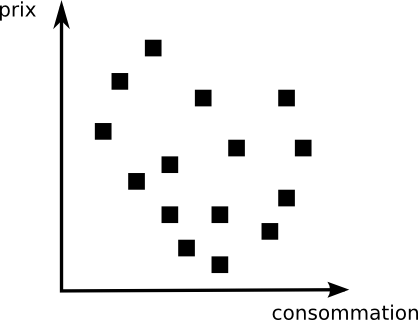
\includegraphics[width=.3\linewidth]{opti1.png}
  	\label{subfig_voiture:a}}\qquad
    \subtop[]{
	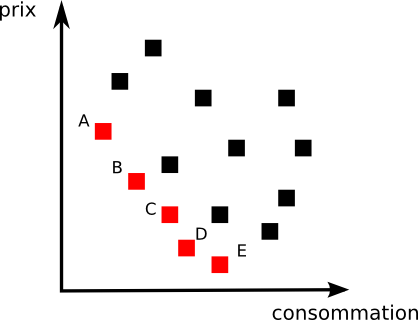
\includegraphics[width=.3\linewidth]{opti2.png}
  	\label{subfig_voiture:b}}
    \subtop[]{
  	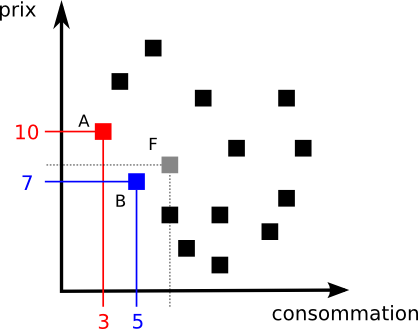
\includegraphics[width=.3\linewidth]{opti3.png}
  	\label{subfig_voiture:c}}
 \end{sidecaption}
\end{figure}

\sloppy En regardant en détail les capacités des voitures figurant dans ce front \ref{subfig_voiture:c}, on voit bien que chacune d'entre elle domine une partie des autres voitures sur au moins un des deux objectifs. Si on prend le cas de la voiture F, celle-ci n'est pas dans pris en compte dans les solutions optimums, car le point est dominé sur ses deux objectifs par d'autres voitures : $ prix(B) < prix(F) < prix(A) $ et $consommation(A) < consommation (B) < consommation(F)$.

Le front de Pareto renvoie un ensemble de solutions compromis optimal, l'expertise finale sur la ou les solutions à adopter est donc le résultat d'un choix expert externe introduit comme support à l'algorithme optimiseur. Dans notre exemple, l'acheteur devra pour finaliser son achat mettre en avant au moins un des deux critères afin de départager les voitures.

Si certains algorithmes ont introduit cette expertise par le biais d'une sélection interactive guidant l'optimiseur à chaque étape de sa recherche, ce n'est pas cette usage qui nous intéresse ici. L'expertise n'intervient qu'une fois les solutions convergés, dans l'observation des résultats finaux.

Dans notre cas, on considère que l'optimiseur doit sélectionner avec les moyens qu'on lui a fournis les solutions candidates sur lesquels il doit miser pour converger. Il doit donc être capable de séparer les solutions en appliquant un ou plusieurs critères de séparation. Il existe plusieurs types de stratégies (\textit{Agreggation based, Criterion based, Dominance based, Indicator based}), et chacune d'elles peut être croisée ou dérivées en de multiples variantes \autocites[28]{Zitzler1999a, Deb2001}[7]{Liefooghe2009}. Nous limiterons ici notre analyse à un seul de ces cas, en nous focalisant d'ores et déjà sur les méthodes les plus utilisées en EC, basées sur la dominance celles-ci sont directement inspirées des travaux de Pareto.

% TODO : Finir ce paragraphe historique rapide, qui permettra de faire la différence ensuite avec les algorithmes inspirés par Pareto.
% TODO : Ajouter ref de Goldberg sur les sciences humaines + GA dans le chapitre 1

\begin{figure}[!htbp]
	\begin{sidecaption}[fortoc]{Graphique en deux dimensions des fonctions objectifs $f_1$ et $f_2$ du tableau \ref{tab:pranking}}[fig:pranking_a]
		\centering  	
		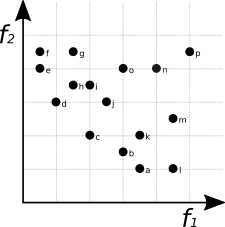
\includegraphics[width=.4\linewidth]{pareto_ranking_a.pdf}
	 \end{sidecaption}
\end{figure}

\begin{table}[!htbp]
\begin{sidecaption}[fortoc]{Tableau de résultats des fonction objectifs $f_1$ et $f_2$ pour un vecteur de solutions candidates $\{a \dotsc p\}$ dans l'espace des objectifs $\mathbb{Y}$, et résultat du \textit{Pareto Ranking}}
	[tab:pranking]
	\centering
	\begin{tabular}{>{$}l<{$}>{$}l<{$} >{$}l<{$} >{$}l<{$}}
			\toprule
			\text{solutions candidates} & f_1 & f_2 & \text{dominé par} \\
			\midrule
			a      & 3.5    & 1    &  \varnothing \\
			b      & 3      & 1,5  &  \varnothing \\
			c      & 2      & 2    &  \varnothing \\
			d      & 1      & 3    &  \varnothing \\
			e      & 0.5    & 4    &  \varnothing \\
			f      & 0.5    & 4.5  &  \{e \}  \\
			g      & 1.5    & 4.5  &  \{d,e,f,h \} \\
			h      & 1.5    & 3.5  &  \{d \} \\
			i      & 2      & 3.5  &  \{c,d,h \} \\
			j      & 2.5    & 3    &  \{c,d \} \\
			k      & 3.5    & 2    &  \{a,b,c \} \\
			l      & 4.5    & 1    &  \{a \} \\
			m      & 4.5    & 2.5  &  \{a,b,c,k,l \} \\
			n      & 4      & 4    &  \{a,b,c,d,e,h,i,j,k,o \} \\
			o      & 3      & 4    &  \{b,c,d,e,h,i,j \} \\
			p      & 5     & 4.5   &  \{a,b,c,d,e,f,g,h,i,j,k,l,m,n,o \} \\
			\bottomrule
	\end{tabular}
  \end{sidecaption}
\end{table}

Pour comprendre comment cette stratégie et définir mathématiquement la notion d'optimum de Pareto, il faut introduire la notion de \textit{dominance} sur lequel elle s'appuie. Pour cette tâche on s'appuie sur les définitions données par \textcite[65]{Weise2011} :

\foreignquote{english}{An element $x_1$ dominates (is preferred to) an element $x_2 (x_1 \dashv x_2)$ if $x_1$ is better than $x_2$ in at least one objective function and not worse with respect to all other objectives.} 

Ce qui dans le cas d'une minimisation se traduit mathématiquement par les conditions suivante : 

\begin{align*}
	(x_1 \dashv x_2) \Leftrightarrow &\forall i \in 1 \dotsc n \Rightarrow - i f_i (x_1) \leq i f_i (x_2) \land \\
	&\exists j \in 1 \dotsc n : j f_j (x_1) < - j f_j (x_2)
\end{align*}

Cette notion de \textit{domination} ($\succ$) \Anote{notation_dominance} permet de dégager ces trois possibilités

\begin{itemize}
\item $x_1$ domine $x_2$ , qui peut également s'écrire $x_1 \succ x_2$
\item $x_1$ est dominé par $x_2$
\item $x_1$ n'est pas comparable avec $x_2$
\end{itemize}

Celle-ci possède les propriétés suivantes, qui définissent dans l'espace des objectifs $\mathbb{Y}$ un \textit{strict partial order} : 

\begin{enumerate}
\item{\textbf{non reflexive}}  $x_1$ ne peux pas se dominer lui même
\item{\textbf{non symétrique}} $ x_1 \succ x_2$ n'implique pas $x_2 \succ x_1$, alors que l'opposé est vrai, $x_1 \succ x_2$ implique $x_2$ ne domine pas $x_1$
\item{\textbf{transitive} }
\end{enumerate}

Différents degrés de dominance ont été développés, comme par exemple la notion de \textit{strong dominance} : $x_1$ domine fortement $x_2$ ($x_1 \succ \succ x_2$) si $x_1$ est strictement meilleur que $x_2$ sur tout ses objectifs. 

Pour bien comprendre comment se construit l'ensemble $X^*$ de solutions non dominées $x^* \in \mathbb{X}$ ,on peut étudier en détail comment la dominance se calcule entre les points $e$ et $f$ présentés sur la figure \ref{fig:pranking_a}.

\begin{table}[!h]
	\centering
	\begin{sidecaption}[fortoc]{Application des règles de dominance aux points $e$ et $f$. \\ \\
		   \begin{tabular}{>{$}l<{$}>{$}l<{$} >{$}l<{$}}
					\toprule
					 & f1 & f2 \\
					\midrule
					e      & 0.5    &  4   \\
					f      & 0.5    & 5,5  \\
					\bottomrule
			\end{tabular}\\ \\ 
			(a) $e \succ f$ car e est bien le meilleur sur au moins un des deux objectifs, et n'est pas pire sur aucuns des autres objectifs ($e \succeq f$ ) \\ 
			(b) f ne domine pas e car f n'est pas meilleur sur aucun des deux objectifs et il est pire sur au moins un des deux objectif}[tab:pranking]
		
		\begin{minipage}{0.5\textwidth}
			\centering
			\subbottom[e est dominé par f ?]{
				\begin{tabular}{>{$}l<{$}>{$}l<{$} >{$}l<{$}}
					\toprule
					    & f1 & f2 \\
					\midrule
					e \leq f & \text{true} & \text{true} \\
					e < f   & \text{false}  & \text{true} \\
					\bottomrule
				\end{tabular}
		 	\label{pranking_a}}
		 \end{minipage}\hspace{1em}
		 \begin{minipage}{0.5\textwidth}
		 	\centering
			\subbottom[f est dominé par e ?]{
				\begin{tabular}{>{$}l<{$}>{$}l<{$} >{$}l<{$}}
					\toprule
					  & f1 & f2 \\
					\midrule
					f \leq  e & \text{true} & \text{false} \\
					f < e  & \text{false}  & \text{false} \\
					\bottomrule
				\end{tabular}
			\label{pranking_b}}
		\end{minipage}
  \end{sidecaption}
\end{table}

Les solutions admises parmi le front de Pareto (voir figure \ref{fig:frontoptimal}) sont donc ici toutes celles qui ne sont pas dominées faiblement ($\succeq$), ce qui revient à exclure les points $f$ et $l$ du front optimum $\{a,b,c,d,e\}$ car ils sont dominés faiblement ($e \succeq f$); alors que dans le cadre d'une dominance forte ($\succ \succ$), ceux-ci auraient fait partie du front $\{a,b,c,d,e,f,l\}$. En effet si on prend toujours le cas de $e$ et $f$, la condition testant que $e$ est strictement meilleur que $f$ sur tous les objectifs n'est pas remplie. %Cet ensemble de cardinalité forcément inférieure ou égale est qualifié \enquote{d'ensemble fort non dominé} (\textit{Strongly non dominated set}).

\begin{figure}[!htb]
	\begin{sidecaption}[fortoc]{Tracé du front optimum à partir du calcul des individus non dominés, cf. l'ensemble vide $\varnothing$ dans le tableau \ref{tab:pranking}}[fig:frontoptimal]
		\centering
		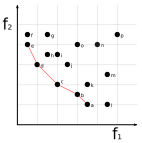
\includegraphics[width=.4\linewidth]{pareto_front.pdf}{
		}
  \end{sidecaption}
\end{figure}

Le front de Pareto n'est en général jamais entièrement couvert, cela pour diverses raisons : 

\begin{itemize}
\item L'évaluation de la fonction à optimiser est souvent coûteuse, comme dans le cas de modèle de simulation dont l'exécution peut prendre jusqu'à plusieurs dizaines de minutes, 
\item La zone d'exploration est volontairement bornée du fait des objectifs des expérimentateurs, 
\item La stochasticité oblige l'exécution de nombreuses réplications d'une même évaluation,
\item On dispose de ressources finies, or l'espace du front est souvent continu et non borné en dehors des contraintes que l'on aura nous-mêmes fixées.
\end{itemize}

Selon \textcite[70]{Weise2011} et \autocite[19]{Zitzler1999a}, on peut s'aider dans cette tâche d'établissement d'un front de Pareto correct en étant attentif aux points suivants:

\begin{enumerate}
\item{\textbf{Proximité}} Les solutions découvertes doivent être les plus proches possibles du front de Pareto optimal.
\item{\textbf{Diversité}} Si le front optimal possible est trop large, la répartition des solutions \textit{spread} doit être maximisé sur toute la surface de celui-ci, si possible suivant une distribution uniforme.
\item{\textbf{Pertinence}} Les solutions découvertes doivent correspondre aux intérêts définis par le problème, et n'ont aucun intérêt si l'opérateur humain ne peut, ou ne sait les utiliser.
\end{enumerate}

On retrouve dans ces objectifs la tension entre exploration et exploitation, le front de Pareto devant être exploité de façon homogène, tout en garantissant à terme (et si possible le plus vite possible) la convergence vers une zone d'intérêt pour l'expérimentateur (voir figure \ref{fig:convergence_diversite}). Les métaheuristiques n'ayant pas d'apriori sur la forme de problème abordée, c'est dans l'originalité, la diversité des constructions proposées qu'une solution optimale et dédiée peut être trouvée. Il est donc très difficile de faire un listing des meilleures stratégies, et des meilleures combinaisons de stratégies permettant une sélection garantie des meilleurs candidats en fonction de ces objectifs, l'établissement de cette liste ne pouvant être que contextuelle d'un problème d'optimisation donné. 

\hl{ref no free lunch theorem }? Wikipedia : Le théorème du « no free lunch » explique qu’aucune instance de métaheuristique ne peut prétendre être la meilleure sur tous les problèmes. Une métaheuristique (M) n’est performante que pour une classe de problème (P) donnée.

Heureusement, un certain nombre de combinaisons, souvent éprouvées par de multiple tests sur des fonctions aux caractéristiques et difficultés soigneusement étudiées (ZDT, etc.), se démarquent par des capacités de résolution acceptable. C'est d'ailleurs souvent sur cette première base que se construisent ensuite les améliorations nécessaires à une réponse optimale, cela en partie grâce à la flexibilité des composantes caractéristique des métaheuristiques. 

\begin{figure}[!htbp]
  \begin{sidecaption}[fortoc]{Convergence et maintien de la diversité au sein du front de Pareto}[fig:convergence_diversite]
  \centering
  \subbottom[Un front de pareto sans maintien suffisant de la diversité]{
  	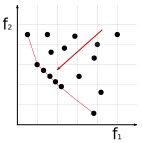
\includegraphics[width=.4\linewidth]{pareto_convergence_a.pdf}
  	\label{subfig_convergence_diversite:a}}\qquad
  \subbottom[Un front de pareto avec maintien de la diversité]{
	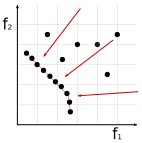
\includegraphics[width=.4\linewidth]{pareto_convergence_b.pdf}
  	\label{subfig_convergence_diversite:b}}
 \end{sidecaption}
\end{figure}

\textit{Une fois défini cet ordre partiel entre les solutions candidates évaluées, sur quelle base l'optimiseur prend sa décision pour sélectionner les individus les plus prometteurs ? et comment celui-ci garantit l'évolution des solutions candidates selectionnées au regard des trois objectifs fixés ?}

Comme le dit de façon très claire,\textcite[94]{Weise2011} \foreignquote{english}{Such comparisons, however, only state whether one candidate solution is better than another one or not, but give no information on \textbf{how much} it is better or worse and \textbf{how interesting} it is for further investigation. Often, such a scalar, relative measure is needed.}

L'optimiseur n'ayant pas les capacités pour comparer des fonctions entre elles, c'est par l'attribution d'un scalaire caractérisant chaque vecteur $z^* \in \mathbb{Y}$ résultat de l'évaluation d'une solution candidate, que celles-ci vont pouvoir être départagées. On parle de \enquote{fonction d'utilité}, ou de \enquote{fonction \textit{fitness}} pour désigner cette opération de transformation dont le résultat $z$ est utile uniquement en se plaçant dans le référentiel de l'optimiseur. Il s'agit d'un classement relatif des solutions les unes par rapport aux autres, calculés indépendamment des valeurs prises par les fonctions objectives, et intégrant un certain nombre d'autres critères, définis en réponse aux exigences des trois objectifs déjà évoqués (respect de la diversité, qualité de convergence, pertinence vis-à-vis du problème). 

Ainsi, un des tout premiers paramètres à intégrer dans le calcul de cette fonction \textit{fitness} tient évidemment dans le choix d'une stratégie pour tirer un meilleur partie des informations récoltées dans l'application de cet ordre partiel sur l'espace $\mathbb{Y}$. Là ou des algorithmes vont appuyer la sélection des solutions à partir d'un calcul de rang (je ne garde que les $n$ premiers rangs), d'autres vont le faire à partir d'un décompte des non dominés (je ne garde que les individus non dominés $< n$), à partir d'une profondeur (je ne garde que les $n$ premiers fronts), ou encore en mélangeant ces trois informations (voir le résultat du calcul de ces trois informations dans \ref{tab:pranking} \hl{a finir}) A cela il faut également ajouter la diversité de choix à disposition dans la selection d'une dominance, par le changement de l'opérateur utilisé dans le calcul (\textit{weak dominance}, \textit{strong dominance}, etc.), ou même la relaxe de celui-ci (\textit{epsilon-dominance}). Des choix de première importance, car ils interviennent directement dans la construction de l'ensemble de solution retenue.

C'est donc dans l'espace des objectifs $\mathbb{Y}$ que se révèle la première information pertinente pour l'optimiseur, nous indiquant, peu importe la forme de l'une ou de l'autre des fonctions et le positionnement des points sur celles-ci, une première sélection de solutions parmi les solutions candidates évaluées sur laquelle l'effort de l'optimiseur doit porter en priorité.

Mais lorsque l'on reprojette les résultats du front de Pareto dans l'espace figurant la dynamique supposée de chacune des deux fonctions objectifs, on observe que la prise de décision basée sur le seul ordonnancement des solutions n'est pas suffisante pour garantir une selection optimale des meilleurs candidats à l'évolution (voir figure \ref{fig:mo_landscape}). 

La forme des fonctions dans cette figure est représentée en pointillé car elle n'est qu'une description temporaire d'un paysage en partie inconnu, en attente d'être révisée par l'évaluation de nouveaux points. Le tracé d'un paysage ne se confond plus comme cela pouvait être le cas dans une optimisation mono-objectif avec la valeur prise par la fonction objectif, et doit maintenant intégrer un intermédiaire supplémentaire plus complexe qui est le calcul d'une fonction \textit{fitness}, et dont la formulation, dépendante de nombreuses stratégies, va modifier les solutions choisies dans le futur, et donc modifier la façon dont on va découvrir l'approximation de ce paysage, cela de façon indépendante aux objectifs choisis. \autocite{Weise2011}

\begin{figure}[!htbp]
	\begin{sidecaption}[fortoc]{Projection du front de Pareto optimal (point \sqbox{tangoBlack1}), et des autres solutions candidates dominées (point \sqbox{tangoGrey1}) sur l'espace de variation du paramètre $x \in \mathbb{R}$, un schéma inspiré par \textcite[67]{Weise2011}
	\parbox{\marginparwidth}{
	\begin{enumerate}[label={},labelindent=0pt,leftmargin=*]
	      \item \sqbox{tangoBlue1} $f_{1}(x)$
	      \item \sqbox{tangoRed1} $f_{2}(x)$
	\end{enumerate}}\\
	Les fonctions $f_{1}(x)$ et $f_{2}(x)$ sont représentées en pointillé car elles sont inconnues de l'optimiseur, et ne servent que de repère au lecteur pour mieux comprendre comment un paysage caractérisant l'intersection des deux fonctions peut émerger durant l'optimisation, et pourquoi cela peut être intéressant d'intégrer son analyse à l'optimiseur.}[fig:mo_landscape]
	 \centering
	 	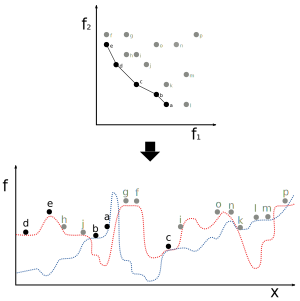
\includegraphics[width=0.8\linewidth]{multi_objective_landscape.pdf}
	\end{sidecaption}
\end{figure}

%on se rend également compte qu'un surplus d'information tiré de l'exploitation d'autres espaces pourrait être utile au choix de l'optimiseur

%\Anote{weise_multi2D}
Déjà beaucoup plus difficile à imaginer que dans l'exemple précédent de l'équation de Schaeffer, la re-projection des solutions candidates évaluées se fait sur un nouvel espace $\mathbb{G}$ (voir figure \ref{fig:relation_espaces}), qui inclu l'ensemble de tous les éléments $g \in \mathbb{G}$ qui peuvent être manipulés par les opérateurs de recherche à disposition de l'optimiseur \autocite[82]{Weise2011}. Un processus détaillé un peu plus tard dans cette section.

Dans notre cas $x \in \mathbb{R}$, on a donc un paramètre qui est manipulable et peut prendre une infinité de valeurs dans le cadre des contraintes définies pour $x$ (par exemple une valeur de 0 à 10 pour $x$) \Anote{remarque_resolution}. L'espace $\mathbb{G}$ contient la codification du problème, ce qui par exemple dans le cadre de simulation, se traduit pour chaque élément $g$ par l'attribution d'un vecteur de paramètres définissant les entrées de la simulation sur lequel l'optimiseur va pouvoir \enquote{jouer} pour optimiser les différentes fonctions objectifs.

La fonction $gpm : \mathbb{G} \mapsto \mathbb{X}$ est une translation opérée lorsque les deux espaces sont de nature différente, par exemple pour passer d'un espace Binaire à un espace de Réels $\mathbb{B} \mapsto \mathbb{R}$. Dans le cadre de simulations, les deux espaces sont souvent de nature similaire $\mathbb{G} = \mathbb{R}$. On pourra se référer à \textcite[86-88]{Weise2011} pour plus de détails.

\begin{figure}[!htbp]
	\begin{sidecaption}[fortoc]{Résumé des relations entre les différents espaces dans une optimisation}[fig:relation_espaces]
		\centering
		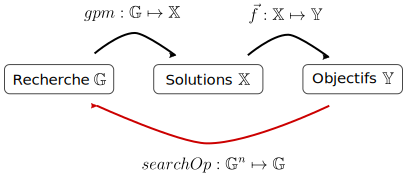
\includegraphics[width=.7\linewidth]{objectifsToSearchSpace.pdf}
  \end{sidecaption}
\end{figure}

%D'une part, l'observation de dynamiques en partie contraires sur ces deux fonctions $f_1$ et $f_2$ nous permet de constater encore une fois pourquoi un déplacement de l'optimiseur sur l'une ou l'autre des fonctions dirigé par la recherche d'un optimum n'a aucun sens. 

L'opération de sélection des solutions candidates est souvent rattachée au processus de convergence. L'objectif de l'optimiseur est d'évaluer au mieux le potentiel de chacune des solutions durant cette phase de sélection pour intégrer et conserver les meilleurs éléments à son référentiel entre deux itérations. On imagine pourtant très bien bien l'effet que peut avoir une sélection trop restrictive sur le maintien de la diversité. C'est le cas par exemple si l'optimiseur ne décide de garder que le front de Pareto, on voit bien sur la figure \ref{fig:mo_landscape} à quel point la couverture de la dynamique des deux fonctions ressortirait considérablement appauvrie à la suite d'un tel choix. On en déduit que la frontière entre stratégies de convergence, et stratégie de maintien de la diversité doit être assez perméable pour garantir le choix de solutions candidates pertinentes en dehors du seul front de Pareto. Zitler \hl{ref autre que ppt à trouver} retient par exemple parmi ces classes de stratégies celle s'appuyant sur le couple associant espace des objectifs et au choix la dominance, la densité, le temps, ou encore la chance. Ce sont des heuristiques qui vont intervenir en amont sur la qualité et la diversité des solutions candidates (par exemple les stratégies de \textit{sharing}, \textit{crowding}, etc.) qui peuvent ensuite être manipulées par les opérateurs de recherches de l'optimiseur.

Viennent ensuite les stratégies de recombinaison des solutions selectionnées, créatrices de nouvelles solutions candidates à évaluer. Un processus qui peut être là aussi rattaché tout autant au maintien de la diversité qu'à une volonté de convergence accrue. Il n'y a là encore aucune règle d'applications spécifique, et tout dépend de l'objectif fixé de façon initiale ou au cours de l'expérimentation. Ainsi, certaines stratégies intégrés aux opérateurs peuvent être mis en place pour limiter une convergence trop rapide des solutions (\textit{premature convergence}) liée à une perte de diversité, alors que d'autres vont tenter d'accélérer cette convergence par la mise en oeuvre d'opérateur de recherche plus agressif, soit pour trouver le plus rapidement possible un minimum (ou maximum) local, soit car la topologie de l'espace des objectifs est de topologie difficile. 

La sélection de candidats à la manipulation dans l'espace des objectifs $\mathbb{X}$ se réfère, une fois projetée dans cet espace $\mathbb{G}$, aux éléments $g$ accessibles à la manipulation par les opérateurs de recherche de la fonction $searchOp$. Chacun de ces opérateurs, dont le nombre et la nature est un paramètre de l'optimiseur, s'appuie sur la transformation d'une ou plusieurs solutions candidates dirigée par la création d'un nouvel élément $g$, dont on attend si possible un meilleur résultat à l'itération suivante. Un postulat très fort est posé par ce type de méthode d'optimisations, l'introduction de petites variations sur les valeurs de l'espace de recherche est également censée apporter de petites variations dans l'espace des objectifs, que cela soit en bien, ou en mal. Appelé \textit{strong causality} \Anote{note_strong}, cette propriété est évidemment dépendante de la forme prise par le paysage du problème (\textit{problem landscape}), et plus celui-ci est accidenté, rugueux, plus sa résolution est considérée comme complexe \Anote{note_weak}.

En relation avec cette observation, l'éclatement de cette population de solutions candidates évaluées sur le paysage nous permet de constater (voir la figure \ref{fig:mo_landscape}) à quel point la notion de distance entre les points parait différente entre ces deux espaces. $f$ et $c$ apparaissent ici beaucoup plus proche de trouver un optimum global que $a$ et $b$, pourtant plus proche de $c$ dans l'espace des objectifs. On voit bien ici que la sélection de solutions candidates intéressantes peut intégrer d'autres informations utiles, en supplément de celle fournit par l'analyse de $\mathbb{Y}$, au travers de l'analyse de cet espace $\mathbb{G}$; et cela toujours afin de guider au mieux l'optimiseur dans la selection des candidats à l'évolution. Un croisement du positionnement des individus $f$ et $c$ donnerait ainsi une bien meilleure valeur de $x$ à évaluer, probablement meilleure que celle d'un individu $a$ et $c$. Si la solution $f$ avait été éliminée sur le fait d'une sélection aux critères plus drastiques, c'est aussi la possibilité d'un croisement fructueux avec $c$ qui disparait.

%A ces stratégies principales s'ajoute un autre ensembles de stratégies, dont certaines sont plus spécifiques, ou constitutives des types d'algorithmes utilisés. %Le maintien d'une diversité de solutions entre les itérations fait partie de ces stratégies qui font partie d'un set plus large de stratégies permettant de contrer l'émergence des différentes difficultés (stochasticité, topologie, etc.) caractéristique d'un problème de résolution unique. 

%Généralement nommé \foreignquote{english}{Pareto Ranking} \Anote{utilisation_pareto_ranking} aussi nommé par Weise \foreignquote{english}{Prevalence Ranking}.

% Ou introduire la notion d'individu ?

\begin{figure}[!ht]
	\begin{sidecaption}[fortoc]{Résumé simplifié du déroulement d'une optimisation selon \textcite[109]{Weise2011}}[fig:resume_opti]
		\centering
		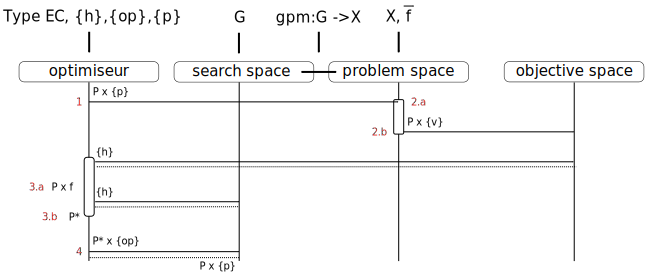
\includegraphics[width=\linewidth]{espace_resume.pdf}{
		}
  \end{sidecaption}
\end{figure}

\hl{Commentaire et schéma pas tout à fait finis}

La description des étapes de la figure résumé \ref{fig:resume_opti} sont les suivantes :

\begin{itemize}[label=\textbullet]
	\litem{1} Une première population $P \in {1 \dotsc n}$ de vecteur paramètres ${p}$ est généré par l'optimiseur ou introduite par l'expérimentateur, puis soumis à évaluation.
	\litem{2.a} La fonction à optimisé est évalué autant de fois qu'il y a de vecteurs ${p}$ 
	\litem{2.b} Les fonctions objectifs $\vec{f}$ sont calculés, ce qui permet de créer autant de vecteur ${v}$ correspond au résultats des fonctions qu'il y a de $P$ évalué. Ces vecteurs $P(v)$ peuvent être positionné dans un espace des objectif $\mathbb{Y}$ 
	\litem{3.a} Le calcul de fitness $f$ est effectué pour chaque élément de $P$ en utilisant les informations rapportés par un ensemble d'heuristiques sur $\mathbb{Y}$ et, ou $\mathbb{G}$
	\litem{3.b} A partir du calcul de cette fitness $f$ pour chacun des éléments de $P$, on selectionne les $P^*$ meilleurs éléments.
	\litem{4} A partir d'un ensemble d'opérateur ${op}$ on va générer de nouveaux vecteurs de paramètres $P(p)$, qui va constituer le nouveau jeu de solution candidates à évaluer à l'étape (1), et dont on espère qu'elles seront si possible meilleures que les précédentes.
\end{itemize}

\hl{Manque la notion d'invididu = fitness + genotype + phenotype}

% Injection de connaissance se fait un peu partout pour la construction d'une fitness.

% Penser à dire qu'il y a plusieurs stratégies de comparaison autre que Pareto ? 

%Première fois utilisé en 1989

%Si on transfère ce langage neutre au vocabulaire que l'on peut trouver courrament dans l'EC, alors l'espace des solution devient le \textit{phenome}, et le point de cet espace qui correspond à la solution candidate devient un \textit{phenotype}.

%\begin{figure}
%\begin{sidecaption}[fortoc]{ POM cycle for developping theory for an agent behavior \autocite[245]{Railsback2012}}[fig:S_syntheseGrim]
%  \centering
% 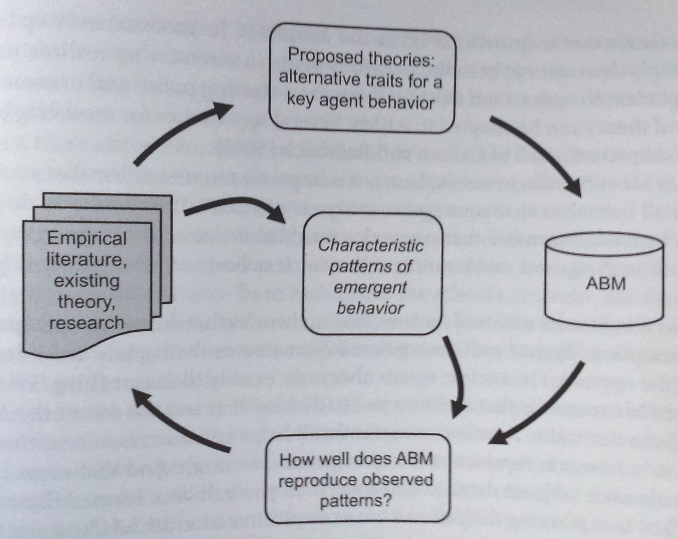
\includegraphics[width=.9\linewidth]{cyclePOMcomportement.png}
%  \end{sidecaption}
%\end{figure}


%Dans notre étude, l'objet à optimiser ne se réfère pas à une expression mathématique, mais à un modèle de simulation, sur lequel on va déterminer un ensemble de critères qui vont faire figure d'équivalent de ces fonction objectives. Dans ce cas d'utilisation, l'optimisation est plus souvent employé comme une forme de calibration inversé \autocite{Grimm2011}, dans laquelle on cherche à déterminer si il existe un ou plusieurs jeu de valeur de paramètres du modèles de simulation respectant la plage de valeur viable empiriquement qui permettent de maximiser l'obtention d'un ou de plusieurs critères experts. Il est plus parlant dans notre cas de désigner l'espace de recherche comme l'espace des paramètres.  

La branche des métaheuristiques EC que nous allons étudier plus spécifiquement s'appuie sur l'observation de phénomènes naturels, comme l'évolution, ou l'organisation, pour la construction et la mise en oeuvre d'algorithmes mimant certaines propriétés intéressantes de ces processus, cela sans être rattaché à une contrainte de réalisme biologique.

\subsection{Les métaheuristiques bio-inspirées, la branche des Algorithmes Evolutionnaires}

\subsubsection{Un rapide historique de la discipline}

On a déjà rapidement décrit dans la section à propos de l'Artificial Life \ref{p:heritage_complexe} les deux voies qu'il était possible d'emprunter dans l'intéret porté sur la définition du processus naturel d'évolution. 

Il existe en effet au moins deux façons aujourd'hui d'introduire des développements informatiques se rapportant à ce processus évolutif. D'un côté, les tentatives de reproduction plus ou moins fidèles des différents mécanismes à l'oeuvre dans le processus d'évolution mettent en avant un objectif de compréhension, alors que la focalisation sur ces mêmes mécanismes pour leur seule capacité d'apprentissage tend à s'éloigner de la réalité biologique pour s'orienter plus vers le développement d'algorithmes désignés comme métaheuristiques. Autrement dit, là ou des chercheurs vont tenter de reproduire au mieux le processus d'évolution dans ce qu'il a de créatif, de non optimisé, de coévolutif car construit par \Anote{note_pattee_semantic_closure} et avec l'environnement, d'autres vont reprendre ce même processus en vue d'une évolution si possible bornée et dirigée par la résolution efficace d'un ou de plusieurs objectifs définis de façon fixe et extrinsèque \autocites{Taylor2001, Taylor2012}.

Lorsqu'on s'intéresse de plus près à la littérature scientifique de ces algorithmes regroupés depuis Fogel sous le terme d'\foreignquote{english}{Evolutionary Computation} (EC), on constate pour toute une partie des publications une de-contextualisation complète de leur utilisation. La question d'une similitude initiale avec le vivant n'étant le plus souvent évoquée que pour illustrer des racines historiques éloignées. Ce qui peut apparaitre comme une forme de surspécialisation est en quelque sorte le prix à payer d'une évolution de la discipline avant tout dirigée par une communauté de chercheurs informatiques motivés par la recherche d'algorithmes performants et d'applications génériques.

Si aujourd'hui on peut observer un tel cloisonnement, un regard sur l'histoire de la discipline tend à montrer tout l'inverse, car nombreux sont les pionniers ayant développé des intérêts simultanés pour ces deux approches : les expériences très longtemps restées inconnue du mathématicien Barricelli dès 1954 \Anote{barricelli_multi_utilisation}, l'approche du généticien \textcite{Fraser1957} qui décrit et simule l'évolution de population génétique dès 1957 \Anote{fraser_comment}, les travaux de Pattee et Conrad avec EVOLVE à la fin des années 1960 \autocite{Conrad1970}, les algorithmes génétiques \Anote{holland_multi_utilisation} de Holland, un élève de Burks, un scientifique dont on a déjà vu dans le paragraphe \ref{p:va_automate_cellulaire} qu'il était proche de Von Neumman.

Il existe toutefois une littérature scientifique parallèle qui continue de motiver la rencontre autour de disciplines scientifiques ayant un intérêt pour la recherche en \textit{Artificial Life}. C'est le cas par exemple de la biologie, ou de l'écologie \autocite{Hamblin2013} qui organisent autour de publications transverses la réflexion sur la reintroduction des outils tel qu'ils sont développés en informatique, entrainant de fait aussi la création et l'évolution de ces derniers \autocite{Hogeweg2011}. C'est également le cas en biologie, ou on imagine l'importance que peuvent avoir les travaux de \textcites{Taylor2001}[221]{Taylor1999} pour la mise en oeuvre de modèles de simulation dirigés vers l'émergence \enquote{créative} de nouveaux phénotypes dans un environnement ouvert \autocite[33]{Taylor1999}. Une critique récurrente adressée aux modèles d'auto-organisation actuels \autocite{Pumain2003}, encore incapables de simuler l'émergence de nouvelles structures, de nouvelles entités de façon crédible. Une autre forme de relation entre les deux approches est également envisageable dans certaines disciplines, comme en écologie, où celles-ci peuvent parfaitement se côtoyer : \foreignquote{english}{The first of these requires the application of the evolutionary process in much the same way as it has been traditionally applied within A-Life: as a means to dynamically adjust agent parameter values to support their viability and reproduction within the virtual environment. [...] The second approach we suggest employs artificial evolution to match simulation patterns against data gathered from the level of specific species up to data concerning specific ecosystems. Once the parameters of the system have been optimised so as to reproduce the patterns observed in field data, the evolution algorithm is turned off. The model may then be employed to answer questions relating to the specific ecosystem and species that it represents. Unfortunately it may not then be used to study the evolution of these specific species in specific environments. This is a shortcoming of the artificial evolution algorithm (it does not model real evolution in detail) that would be worth overcoming.} \autocite{Dorin2008}

Le lecteur souhaitant obtenir une vue plus globale des différents concepts et ramifications disciplinaires réunit sous le terme parapluie d'\textit{Artificial Life} peuvent se référer à l'article d'\textcite{Aguilar2014} qui concentre un grand nombre d'entrées bibliographiques essentielles pour aborder les entrées de cette thématique dans chacune des disciplines. On trouvera également une description plus précise sur l'histoire commune de ces deux voies de recherches, telles quelle est perçues par les acteurs historiques de l'EC, dans les ouvrages de \autocites{DeJong2006a, Fogel1998, Fogel2006a, Fogel2006b, Back1996, Back1997}.

Dans cette section, c'est bien la deuxième branche de recherche qui est suivie, celle visant l'\enquote{optimisation}. Les développements tels qu'ils sont abordés ne se mesurent donc plus en fonction d'un critère de réalisme biologique, mais en fonction de critères informatiques et mathématiques se rapportant plus à la capacité de résolution des algorithmes, et aux supports de mise en oeuvre et de mesure de ces derniers : rapidité, diversité, robustesse, qualité, etc.

\textcite{DeJong2006a} retient trois foyers importants pour le développement de cette deuxième branche dans les années 1960, la \textit{Technical University} de Berlin avec Rechenberg, Biernet et Schwefel \autocite{Beyer2002}, UCLA à la même période avec Lawrence J. Fogel, et l'université du Michigan avec John Holland.

De ces trois branches vont émerger au cours des années 1970 ce que \textcite{DeJong2006a} qualifie comme des \foreignquote{english}{Evolutionary Algorithms (EA)} canoniques. Autrement dit, ce sont des algorithmes matures, qui ont prouvé leur capacité à produire des solutions dans un contexte précis : \foreignquote{english}{Evolutionary Programming (EP)}, \foreignquote{english}{Evolution Strategy (ES)}, \foreignquote{english}{Genetic Algorithm (GA)}

Ils vont représenter chacun le foyer d'un développement qui va s'accélérer dans les années 1980, avec l'amorce d'une popularisation de ces techniques permises entre autres par l'avènement de capacités de calcul plus conséquentes et la reconnaissance de l'efficacité de ces algorithmes pour la résolution de problématiques industrielles plus concrètes. L'ouvrage de synthèse écrit par \textcite{Goldberg1989} contribue de façon très importante à cette diffusion, et constitue également un apport théorique important dans la naissance de la branche multi-objectif de cette discipline.

Les années 1990 vont quant à elles consacrer la rencontre et l'unification de ces différentes approches restée jusqu'alors assez indépendantes si on en croit \textcite{DeJong2006a}. De cette confrontation nait la reconnaissance d'un seul terme fédérateur, l'\textit{Evolutionary Computation (EC)} motivant alors la création de nouvelles conférences et de nouveaux journaux structurant cette nouvelle discipline. C'est aussi à partir de cette période que l'on observe la mise en place d'une hybridation accélérée entre les différentes approches qui s'accompagne d'une forme de remise à plat théorique et l'émergence d'un cadre de réflexion unifié. \autocites[23-31]{DeJong2006a}{Back1997}

Si on se concentre plus précisément sur la branche multi-objectif de la discipline, la première introduction théorique d'une stratégie s'appuyant sur le calcul de l'optimum de Pareto pour définir un classement original des solutions évalués est présenté à la page 197 de \textcite[197]{Goldberg1989}. Cette technique nommé \textit{Non Dominated Sorting} (NDS) \autocite[40-43]{Deb2001}, probablement la plus efficace et plus célèbre, sera reprise et implémenté presque dix ans plus tard en 1994, dans l'algorithme célèbre NSGA (Non dominated Sorting Algorithm) de Deb et Srinivas.

Les travaux de \textcite{Goldberg1989} ont influencé tout une génération de chercheurs à partir de cette simple ébauche théorique de tri basé sur la dominance de Pareto, et nombreux sont ceux qui se sont par la suite appuyés \autocite[175, 235]{Deb2001} sur les informations du calcul de dominance pour développer diverses stratégies d'attribution de \textit{fitness}, comme MOGA (Fonseca et Flemings 1993), NPGA (Horn et Nafpliotis 1994), NSGA (Deb et Srinivas 1994), et bien d'autres \autocite[14]{Zitzler1999a}. Ce que l'on peut considérer comme la génération suivante d'algorithmes, que \textcite{Coello2006} \Anote{coello_note} fait démarrer avec l'apparition de l'élitisme \Anote{note_elitisme}, est plus axée encore sur l'efficacité de ces derniers avec notamment l'ouverture d'une branche de recherche développant des métriques de performance, et de nouveaux standards de mesures \autocites{Coello2006, Zitzler2003}, dont on s'aperçoit qu'elles sont devenues nécessaires pour comparer correctement les algorithmes entre eux \autocite[14-15]{Zitzler1999a}. Parmi ces nouveaux algorithmes, devenus depuis canonique, on trouve PAES (Knwoles and Corne 2000), SPEA (\autocite{Zitzler1999}), ou encore NSGA 2 (Deb 2000) etc. On trouve à ce sujet un état de l'art et des exemples de calculs à la main pour ces différents algorithmes dans un des premiers et très bon ouvrage de synthèse de \textcite{Deb2001}, aux chapitres 5 et 6. Il est toutefois à noter, comme le fait déjà Golberg en 1989, que cette problématique de recherche d'une solution à un problème multi-critères, puis multi-objectifs est d'origine bien plus ancienne, et a pu servir de support à la mise en oeuvre de techniques plus ou moins similaire à celle de Pareto. Ainsi, les premières traces en EA d'un intérêt théorique et parfois pratique de ces problèmes semblent remonter à Box et Draper (1957), Fogel (1966), Rosenberg (1967) \autocite[174-175]{Deb2001}. Mais la première implémentation informatique est en général attribuée à David Schaffer, avec son travail de thèse (1984) et l'implémentation de l'algorithme d'optimisation VEGA (\textit{Vector Evaluated Genetic Algorithm}). Un autre état de l'art sur l'optimisation multi-objectifs s'appuyant sur Pareto en dehors des techniques purement évolutionnaire est également possible. C'est grâce à l'existence de ce cadre formel mathématique permettant la description d'un problème d'optimisation, tel que nous l'avons un peu abordé dans la section précédente en s'appuyant sur les écrits de \autocite{Weise2011}, que \textcite[50-79]{Deb2001} indique par exemple comment certaines de ces stratégies hors EC ont été pour certaine également transférées avec plus ou moins de succès aux EA \textcite[171-237]{Deb2001}.

Enfin on notera qu'il existe également une autre classe proche d'algorithmes d'optimisation basée sur une observation des mécanismes naturels, celle-ci n'étant plus basée sur la métaphore évolutive par reproduction (même si l'hybridation est envisageable), mais sur les capacités d'organisation et d'auto-organisation observées chez certains animaux comme les fourmis, les abeilles. Ces comportements ont d'abord inspiré les développements de plateformes informatiques adaptées à l'émergence de ce type de comportements, avant d'être repris et utilisé de façon beaucoup plus abstraites par la suite pour résoudre des problèmes d'optimisation. Aujourd'hui regroupées sous le terme de \foreignquote{english}{Swarm Intelligence}, ce sont par exemple les algorithmes PSO (Particle Swarm Optimization), ACO (Ant Colony Algorithms), ABC (Artificial Bee Colony), etc.

\subsection{Les principes sous-jacent aux EA}

Afin de pouvoir mettre en oeuvre la possibilité d'une telle souplesse dans l'adaptation de l'algorithme à une problématique d'optimisation donnée, \textcite[49]{DeJong2006a} a considéré la construction d'un modèle conceptuel plus abstrait capable d'englober dans sa description les mécanismes d'au moins ces trois version canoniques GA, ES et EP. Les concepts clef qui se dégagent d'une telle prise de distance peuvent ainsi être repris non seulement pour décrire les version canoniques mais également pour développer de nouvelles variantes ou extensions d'algorithmes. 

Les éléments communs retenues sont les suivants :

\begin{itemize}
\item Une population de taille constante $m$ évolue au cours du temps
\item La population courante est utilisée comme une source de parents pour produire une progéniture (\textit{offsprings}) de taille $n$
\item La population étendue ainsi constitué est réduites de $m + n$ à $m$ individus.
\end{itemize}

% En général puis recentrage sur les détails ?
\paragraph{Les avantages et les inconvénients d'une terminologie spécifique}

En 2014 une publication sur le blog du spécialiste de la discipline Thomas Weise's \Anote{billet_weise} revient longuemment sur les problématiques de ce vocabulaire inspiré par la biologie et ancré dans les différentes branches composantes l'EC. Il retient quatre problématiques dans l'usage de cette terminologie, parmi lesquels l'incompatibilité des terminologies entre les différentes branches, la dissonance entre la terminologie et la réalité d'application des algorithmes, le fait que l'optimisation au sens naturel n'est pas forcément une bonne optimisation, le fait également que cette terminologie sonne comme anti-profesionelle \Anote{note_pengouin}. Le plus grand problème étant dans ce cadre l'invention de néologisme ne faisant référence ni au domaine biologique, ni au domaine informatique.

Si la perspective d'un changement d'annotation et de vocabulaire est probablement conçu comme une étape majeure dans la progression et l'unification d'une discipline depuis quelques années déjà sur la voie de la maturité, Weise tout en pronant au maximum la bonne parole continue comme beaucoup d'autres à utiliser cette terminologie \autocite{Weise2011}, très ancrée dans un folklore qui tient à l'historique de la discipline. La librairie logicielle MGO décrite par la suite s'appuie elle aussi sur cette terminologie, aussi nous n'utiliserons donc les terminologies alternatives proposés par Weise que sous forme de complément, afin de ne pas introduire trop de distance entre les termes décrivant les algorithmes dans ce manuscrit et la réalité du programme tel qu'il est conçu.


\begin{table}[!htbp]
\begin{sidecaption}[fortoc]{Tableau de correspondance entre les notations à consonnance biologiques et les notations plus génériques liés à l'optimisation, lorsque celles-ci existent. Une traduction appuyée sur la section précédente, et les travaux de \textcite{Weise2011}}
	[tab:ptraduction]
	\centering
	\begin{tabular}{ll}
		\toprule
		générique & biologique (FR)\\
		\midrule
		Espace du problème ($\mathbb{X}$) & Phénome \\
		Espace de recherche ($\mathbb{G}$)   &  Génome \\
		Point dans un espace de recherche ($g \in \mathbb{G}$) & Génotype \\
		Solution candidate, Point dans un espace de solutions ($x \in \mathbb{X}$) & phénotype \\
		Opérateurs de recherches ($searchOp$) & Reproduction \\
		Opérateur de recherche Unaire & Mutation \\
		Opérateur de recherche Binaire & Crossover \\
		Itération & Génération \\
		?  & Progéniture \\
		?  & Mating pool \\
		\bottomrule
	\end{tabular}
  \end{sidecaption}
\end{table}

\paragraph{Les avantages et les inconvénients}

Origine : Deb2001, Fogel2000, Back1997, \autocite[104,105]{DeJong2006a}

\begin{enumerate}[label=(\alph*),labelindent=\parindent,leftmargin=*]
	
	\item Evaluation d'une population entière par génération, ce qui n'est pas le cas de nombre de techniques fournissant une seule solution par execution d'algorithme.
	\item Facile à paralléliser, une propriété étudié très tot, voire \autocite[444]{Alba2002} 
	\item Ne demande a priori aucune connaissance de la forme du paysage, même si en réalité c'est un plus pour bien choisir et paramétrer les métaheuristiques
	\item Applicable à des problèmes continus, discrets, ou les deux.
	\item Ne demande pas forcément de repartir de zéro entre chaque analyse en comparaison à d'autres algorithmes
	\item Le nombre de degré de liberté pour modifier une métaheuristique est très important, ce qui augmente les chances de trouver une combinaison adapté à un problème complexe donné
	\item Les principes de mise en oeuvre sont relativement facile à comprendre
    \item Efficace, même sous une forme canonique
    \item Capacité à explorer de très large espace de recherche
\end{enumerate}

Désavantages, limitations : 
\begin{enumerate}[label=(\alph*),labelindent=\parindent,leftmargin=*]
	\item le fonctionnement reste opaque, et le résultat n'est souvent pas tractable mathématiquement
	\item Stochasticité demande réplication
	\item Non garantie d'un optimum global
	\item Le nombre de degré de liberté demande une certaine forme expertise pour en tirer le meilleur partie, la construction d'un EA optimal pour un problème donné étant progressif, incrémental
    \item Trop facile à comprendre, il en résulte une certain illusion quant au capacité \enquote{magique} de ce type d'algorithme.
    \item Necessite une source conséquente de puissance pour réaliser de grand nombres de calculs en parallèle 
    \item Meme si les résultats sont meilleurs avec ce type d'approche, celle(ci a ses limites, et les performances se dégrade avec l'augmentation de l'espace de recherche (dimensionalité) et ou le nombre d'objectifs (limite de l'approche Pareto) Zitzler1999a page 24 cite Fonseca Flemming 1995
\end{enumerate}

Optimisation de paramètres est un domaine d'application reconnu des EA du fait aussi de la facilité de mapping entre vecteur de paramètres et génome \autocite[83]{DeJong2006a}

Dans la lignée des objectifs définis dans le chapitre 3, cette branche spécifique des EA est celle qui est à la fois la faciles d'accès en terme de compréhension pour les débutants tout en restant également suffisament de flexibilité et d'efficacité pour convenir à notre utilisation. 

De plus certains désavantages sont de conséquences plus limités dans le cadre de nos objectifs. En effet, pour le profil d'utilisateur modélisateur que nous visons la garantie d'un optimum global n'est pas la priorité immédiate en comparaison de l'importance d'accéder rapidement à des premiers résultats via un premier EA générique exécutable, qu'il pourra de toute façon ensuite améliorer du fait de la nature métaheuristique de ces algorithmes. De façon similaire, le fait que le résultat ne soit pas tractable mathématiquement n'est pas vraiment problématique dans le cadre des systèmes complexes, ou ce type d'observation est justement une propriété récurrente des systèmes que l'on cherche à simuler pour mieux les comprendre. 

Enfin, il est important de noter que cette classe d'algorithmes accueille les approches les plus efficaces pour la résolution de problèmes multi-objectifs, une propriété courante des problèmes abordés dans notre discipline, car les modèles de simulation construisent souvent leur crédibilité aux croisements de multiples critères. (\hl{POM, cf problème inverse calibration déjà expliqué plus haut})


\hl{/..../}


\hl{Introduction à un algorithme simplifié, soit sous forme d'algorithme, soit sous forme de schéma}

\begin{algorithm}[H]
 \KwData{this text}
 \KwResult{how to write algorithm with \LaTeX2e }
 initialization\;
 \While{not at end of this document}{
  read current\;
  \eIf{understand}{
   go to next section\;
   current section becomes this one\;
   }{
   go back to the beginning of current section\;
  }
 }
 \caption{How to write algorithms}
\end{algorithm}

Chacun de ces items ouvre quasiment la voie à des sous domaines d'expertises spécifiques. Voici un apercu cumulatif des élements susceptibles de varier d'un algorithme à un autre, et d'une application à une autre, dont certain sont hérités de la nature métaheuristique des EC, puis de la nature spécifique des EA, et enfin de la nature multi-objectifs (*) : \autocite[69,72,115]{DeJong2006a}[264-269]{Weise2011}[91]{Liefooghe2010} : 

\begin{itemize}
\item la stratégie de représentation interne d'une solution 
\item la stratégie d'initialisation et de maintien d'une ou de plusieurs populations
\item les stratégies de sélection des parents pour la reproduction
\item les stratégies de réintroduction des enfants dans la ou les population(s)
\item le groupe d'opérateurs choisi et la stratégie d'utilisation de ces opérateurs dans le processus de reproduction
\item le choix d'une fonction de translation \textit{gpm} entre $\mathbb{G}$ et $\mathbb{X}$
\item (*) les stratégies de préservation de la diversité
\item (*) les stratégies élitiste de selection et de maintien des survivants
\item (*) la méthode d'attribution d'une \textit{fitness} $v$
\item le critère d'arrêt
\end{itemize}

Si cette liste de classe de choix permet de cerner de façon plus globale les questions à se poser lorsqu'on construit ce type d'algorithmes, cette représentation est encore trop vague, trop linéaire, et ne rend pas compte de la plasticité et des contraintes voulu ou imposé par la construction dynamique d'un algorithme véritablement adapté au problème. Les dépendances entre éléments de la liste n'apparaissent pas dans cette représentation, or pour chacun des choix réalisés par l'expérimentateur a lieu un recalcul des degrés de liberté, ce qui entraine l'apparition ou la disparition de nouveaux choix, en fonction des dépendances existantes entre chaque éléments. \Anote{reflexion_DeJong}

Par exemple, le choix d'une représentation interne d'une solution sous forme de vecteur de binaire, réel ou encore mixte, de taille dynamique ou fixe, doublé ou non de paramètres spécifiques de convergence, joue de façon assez logique sur les choix disponibles dans chacunes de ces classes. Ainsi le groupe d'opérateurs choisi pour manipuler ces vecteurs lors de la reproduction ne seront pas les même selon qu'on manipule des éléments Binaires ou Réels.

De plus, il faut imaginer que chaque stratégie est accompagnée de son lots de paramètres associés, et ce n'est qu'à terme d'une construction, lorsque le choix d'une combinaisons d'éléments est actée que la liste de paramètres définitives apparait de façon claire à l'expérimentateur.

Enfin, dans notre cas, où il est question d'utiliser ces algorithmes évolutionnaires en s'appuyant sur toute la puissance informatique disponible, de nombreux nouveaux choix \autocite[221-224]{DeJong2006a} émergent à la lumière des modèles plus poussé de parallélisation des EA. Par exemple la mise en place d'une stratégie de parallélisation en ilôts, dont on verra un peu plus loin qu'elle est optimale pour une utilisation sur une grille de calcul, pose les nouvelles questions suivantes :

\begin{itemize}
	\item quels sont les stratégies de migration des individus entre les différentes populations ?
	\item combien d'ilots sont nécessaires ?
	\item les population initiale des ilots est elle identique ou différente ?
	\item quelle topologie d'ilot est la plus adaptée ?
	\item etc.
\end{itemize}

C'est un aperçu des problèmes que nous tenterons de résoudre avec la construction d'une librairie logicielle à l'architecture originale, couplé avec openMOLE pour gérer la partie parallélisation, et qui sera exposée dans les sections suivantes.

Une partie de la modularité inhérente aux métaheuristiques a déjà pu par chance être saisie dans le développement de nombreuses librairies logicielles, il est alors légitime de se poser la question suivante, pourquoi développer et surtout maintenir une nouvelle librairie ? 

Les raisons de ce choix sont guidées par une observation critique des librairies existantes, et la volonté de satisfaire au mieux les critères évoqués dans le chapitre 3 \hl{ref section}.

Il est question de mettre en place une librairie de construction d'algorithmes évolutionnaires, exposant une syntaxe lisible exposant le schéma interne d'algorithmes connus et des plus efficaces pour résoudre des problèmes d'optimisation. Destiné à un public novice, 


\paragraph{Expression au niveau de l'expérimentation : }

\begin{enumerate}

\item{Besoin de plus de flexibilité ?} 

\end{enumerate}



Qu'est ce qui fait la facilité de prise en main ? Respecter les pratiques existantes, tout en étant offrant des solutions alternatives lorsque le modélisateur en a besoin. 

\paragraph{Au niveau utilisateur, cas d'utilisation orienté vers les métaheuristiques}

\begin{enumerate}

	\item{\textbf{Besoin de plus de flexibilité ?}} L'algorithme évolutionnaires proposé en l'état ne donne pas de bons résultats, le programme doit permettre d'accéder \textbf{facilement} à toute la combinatoire offerte par la variation des différents composants intégrant cette branche des métaheuristiques. 

	\item{\textbf{Besoin de plus de puissance ?}} Fonctionnel sur une machine standard, les algorithmes évolutionnaires doivent pouvoir tirer parti de ressource informatique plus importante de façon locale (multi-coeur) ou distribué (cluster, grille de calcul), et cela en utilisant les méthodes adaptés. Ce passage d'une execution locale à une execution distribué doit être possible \textbf{facilement}.

	\item{\textbf{Besoin de plus d'extensibilité ?}} Je ne trouve pas le composant nécessaire à la construction d'une métaheuristique adapté à mon problème, quels sont les outils mis à ma disposition pour que je puisse ajouter le ou les composants facilement, à moindre cout, sans que l'ensemble du programme ne soit affecté par mes modifications. 

\end{enumerate}

\paragraph{Au niveau utilisateur, cas d'utilisation orienté vers le couplage (simulation - metaheuristique) }

\begin{enumerate}

	\item{} Mon modèle évolue pour changer de plateforme (Netlogo -> Gamma), mais l'optimisation et les paramètres de l'optimisation reste si possible en place et fonctionnel.
	\item{} Existe-t-il une bibliothèque d'expérimentations comportant un ou plusieurs exemple ou patron(s) pour une utilisation du modèle de simulation avec des métaheuristiques ?
	\item{} Comment sont définit les fonctions objectifs ?
	\item{} Comment sont définit les mapping entre paramètres du modèles et représentation interne d'une solution ?
	\item{} Est ce que ces fonctionalités sont accessible par une manipulation interactive ou par le biais de scripts ?

\end{enumerate}

% MODYSS !

\paragraph{Au niveau technique}

- Modulation de l'accès à la puissance informatique indépendante du modèle : Intégré à OpenMOLE, le couplage doit apparaitre comme transparent, tout en restant hautement flexible ce qui suppose l'existence de primitive de plus haut niveau qui assure la partie parallélisation nécessaire à l'usage confortable de tels algorithmes.


- Découpler les plateformes de simulation 
- Supporter différents niveau de parallélisme au niveau des métaheuristiques

- La facilité d'ajout de nouveaux composants
- Une bibliothèque d'algorithmes canonique à disposition
- La documentation 

Dans l'association entre modèle de simulation et métaheuristique : Modalités de jointure entre le modèle de simulation \enquote{tel qu'il est développé} et la librairie d'algorithme évolutionnaire.

- Séparation entre modèle de simulation 
- 

Deux phases ? 
- Usage indépendant
- Usage associé à openMOLE



fait apparaitre l'optimisation comme une étape supplémentaire dans l'expérimentation, 


%BehaviorSearch follows in the tradition of NetLogo [Wilensky, 1999, 2001; Tisue & Wilensky, 2004], and Logo [Papert, 1980] before it, in embracing the twin design goals of “low threshold” and “high ceiling”. By this we mean that the BehaviorSearch tool should be both easy for beginners to learn and use (“low threshold”), while also providing advanced features that will allow expert modelers to engage in cutting-edge research and analysis (“high ceiling”). To be clear, the “low threshold” goal for NetLogo, which aims to support use by elementary school students, is lower than that of BehaviorSearch, which primarily targets NetLogo’s research audience. However, increasingly NetLogo is being used by undergraduates or even high school or middle school students who are developing agent-based models for research projects, and we would like BehaviorSearch to be accessible to these audiences, as well as researchers from various disciplines who are non-expert programmers but have adopted ABM methodologies for their research. Just as NetLogo strives to make the creation of agent-based models accessible to children and novices, BehaviorSearch aims to facilitate model analysis by making search and optimization techniques accessible to all modelers.

State of the Art
Flexibilité

Facilité de parallélisation 
Facilité de construction

\subsection{Un point rapide sur les solutions EC existantes}

Les librairies logicielles permettant la mise en oeuvre d'algorithmes évolutionnaires existent dans de très nombreux langages informatiques. Les \textit{Survey} ou \textit{state of the art} sont régulièrement mis à jour dans cette discipline, et il est inutile de se substituer ici à ce type de travaux en évoquant les avantages et les inconvénients comparés de toutes ces librairies. Le lecteur pourra se référer à l'étude très complètes de \textcite{Parejo2012} comparant selon 271 critères 11 des plus importantes plateformes sur les 33 qu'ils ont identifiés. De notre coté, on se contentera d'illustrer ce que l'on considère comme les principaux défaut du point de vue de notre grille de lecture en selectionnant un ou plusieurs librairies parmis les plus usités.

Un premier filtre permet d'éliminer toute celle qui ne s'adresse qu'à une seule branche des EA, ou qui n'implémente aucun des algorithmes multi-objectifs. 

Un deuxième filtre permet d'éliminer également toute les librairies qui sont intégrés à un logiciel, impossible à utiliser en dehors de celui-ci. Le cas particulier des logiciels de modélisations (simulateurs) intégrant des algorithmes EC sera toute de même abordé afin de situer les limites de ces approches.

Un troisième filtre, 

Afin de satisfaire les objectifs que nous avons fixés, la librairie doit pouvoir fonctionner avec OpenMOLE, car une des tâches de ce dernier va être d'orchestrer de façon transparente la parallélisation de ces algorithmes evolutionnaires, ce qui suppose une interaction assez fine entre les deux outils, et un langage informatique compatible avec Java ou Scala, les langages sur lequel est construits OpenMOLE.


\subsubsection{Les librairies standards}

Apache Commons

\href{http://www.moeaframework.org/}{@MOEAFramework}

\href{http://dev.heuristiclab.com/}{@HeuristicLab 2002 .Net CSharp Microsoft dependent}

\href{http://jmetal.sourceforge.net/}{JMetal (2010)}

\href{http://image.diku.dk/shark/sphinx_pages/build/html/index.html}{Shark machine learning library (c++)}

\href{http://www.tik.ee.ethz.ch/sop/pisa/?page=documentation.php}{PISA (C / C++) 2003}

Paradiseo-MOEO et Paradiseo-PEO (C ++)
Logiciels de l'INRA

\href{http://cs.gmu.edu/~eclab/projects/ecj/}{ECJ (1998) (orienté GP)}

\href{http://opt4j.sourceforge.net/}{Opt4J (Java) 2011}

\href{http://esa.github.io/pygmo/}{Pygmo (Python) PaGMO (C++) (ESA)}

\href{http://jgap.sourceforge.net/}{JGAP}

\subsubsection{Les approches intégrées}

\paragraph{Le {BehaviorSearch} de Stonedahl}

La librairie \textit{BehaviorSearch} developpé par Railsback pour Netlogo intègre une librairie d'algorithme génétique.

Les solutions existantes de couplage, comme le \textit{behavior search} déjà évoqués dans \hl{la section XX}, ne sont pas entièrement satisfaisantes, cela sur plusieurs points déjà évoqués et résumé ci dessous, auquels on rajoute de nouveaux inconvénients propre à la manipulation avancé des métaheuristique : 

a) Le cycle de vie d'un modèle ne se limite pas forcément à l'établissement d'un seul modèle Netlogo, mais plusieurs, et de complexité différentes. Si Netlogo est un outil indispensable de par la force et la rapidité de concrétisation d'une idée scientifique qu'il permet, les scientifiques non développeur peuvent rapidement être piégé par des problématiques tenant plus de la science informatique que de leur domaine initial. 

b) Le niveau de prise en charge de l'expérimentation est insuffisant pour assurer une recherche reproductible au delà du seul modèle. Par là il faut comprendre que le protocole scientifique supportant l'évaluation du modèle de simulation n'est pas accessible, or tout comme le modèle, celui-ci possède sa propre voie de construction, et porte au contact du premier une responsabilité dans l'évolution des choix de sa structure interne. Autrement dit, sans la présence de ces deux supports de connaissances, c'est toute une discussion collective qui est rendu plus complexe, alors même que celle-ci se révèle comme un support important, voire même constitutif de ce processus de validation.

c) Le support du parallélisme en local, c'est à dire sur un ordinateur personnel, même lorsqu'il est associé à des techniques pour réduire le nombres d'éxecution des modèles de simulation (\textit{fitness caching} \autocite[245]{Stonedahl2011a}), ne semble pas suffisants pour une utilisation confortable et répétés d'algorithmes métaheuristiques multi-objectif. Ces derniers pouvant demander pour des modèles relative simple et optimisé jusqu'à plusieurs millions d'executions, résultat d'une accumulation d'expérimentation nécessaire pour la construction et l'évaluation du modèle de simulation \autocites{Schmitt2014, Cottineau2014b}. Le framework théorique QBME (Query-Based Model Exploration) de Stonedhal est intéressant, et ressemble par certains aspects à la méthodologie POM de Grimm, et permet comme dans cette dernière de questionner la progression du modèle sous la forme d'une question inversé par rapport au questionnement plus traditionnel. On ne se demande plus \enquote{Quels comportements vais je obtenir avec ce jeu de paramètres} mais plutôt \enquote{Quels type de paramètres m'a permis d'obtenir (ou de ne pas obtenir) un certain comportement ?}. Ce type d'analyse se base sur la construction de multiples critères d'évaluation, potentiellement contradictoire, questionnant la dynamique du modèle, et qui il me semble, se rattache plus à l'expression d'une analyse multi-objectifs. Or, les algorithmes proposés par le \textit{BehaviorSearch} se limitent pour le moment à des algorithmes mono-objectif que les cas d'utilisation réels risquent de très rapidement mettre en défaut.

d) Le support ne permet pas à l'heure actuelle de jouer \enquote{facilement} avec les briques mises à disposition par les métaheuristiques, ce qui on l'a vu précédemment va à l'encontre de l'esprit de tels algorithmes. Même si une certaine extensibilité du logiciel à été prévu par le concepteur, sa mise en oeuvre demande des connaissances supplémentaires dans un autre langage de programmation que Netlogo (Scala ou Java), ce qui vient encore surcharger un peu plus les prérequis d'un utilisateur débutant qui doit déjà explorer le domaine des algorithmes evolutionnaires.

Même si l'auteur est effectivement d'accord avec le concepteur du \textit{BehaviorSearch} pour dire que cet outil constitue en lui même déjà un grand pas vers la démocratisation de techniques d'expérimentations plus évolués jugés nécessaire pour améliorer les pratiques des débutants, nous pensons qu'il est possible d'aller encore beaucoup plus loin. A ce titre, le couplage que nous visons dans ce projet se rapproche des visions d'avenir évoqués par le concepteur, dont la dernière version du logiciel est daté de 2013 \textcite[295]{Stonedahl2011a} \foreignquote{english}{In the not-so-distant future I envision in a “begin parallel search” button appearing in toolkits like NetLogo that would seamlessly launch dozens or hundreds of simultaneous genetic algorithms searches on a remote grid/cluster, reporting back the most promising results to the user as they are discovered in real-time.} La différence c'est que ce bouton n'est pas envisagé dans Netlogo, car ce n'est pas le propre de cet outil, mais dans un logiciel tel qu'openMOLE, dont la fonction est entièrement dédié à l'execution de tâche en parallèle sur des environnements locaux (un ou plusieurs processus d'une machine), ou distribués (sur une grille de calcul, ou un cluster d'université)

Si on envisage en effet la construction de modèles sur la base d'une alternance régulière entre construction de modèle et évaluation, il est tout à fait possible et même certain que l'expérimentateur sera un jour ou l'autre confronté à une ou plusieurs limitations provenant de la chaine de progression naturelle prévu par les concepteurs de cet outil \foreignquote{english}{Netlogo(for building the model) => Behavior Space (for simple model analysis) => BehaviorSearch (for more advanced analysis and exploration)} \autocite[340]{Stonedahl2011a} ? Quels sont les choix à disposition des modélisateurs débutants ayant expérimenté l'une ou l'autre de ces difficultés ? (\hl{A voir si cela ne remonte pas dans le chapitre 3 pour cloturer la partie netlogo})

En résumé, les librairies déjà intégré au logiciel de modélisation, comme le \textit{BehaviorSearch} de Netlogo, sont limités en termes d'algorithmes, d'accès la puissance informatique nécessaire, et reste lié à un seul support alors même que le modèle peut être amené à migrer de plateforme. On en déduit que cette solution, bien qu'utile pour du prototypage et de l'apprentissage, ne permet pas d'envisager sereinement la construction d'un modèle ou d'une expérimentation plus complexe.

\paragraph{Les algorithmes EC dans Mason}

Le framework de développement de simulation multi-agent MASON, présenté pour la première fois en 2003, (Multi-Agent Simulation Of ...) tient d'un effort conjoint entre la section d'Evolutionary Computation du laboratoire de science informatique et le \textit{Center for Social Complexity} tout deux de la George Mason University. Ecrit en Java, solidement documenté, de développement ancien, associé depuis les débuts à un laboratoire spécialisé auteur d'une librairie datant de 1998 dédié aux EC nommé ECJ (1998), les deux logiciels étant développés par les même personnes et régulièrement mis à jour ... ce framework apparait au premier abord comme un challenger sérieux pouvant se substituer à Netlogo sur des projets plus complexes. 

MASON se situe sur la même ligne de développement que les librairies de développement multi-agents plus anciennes comme Swarm, Ascape, ou Repast. Tout comme ces dernières, la généricité, la performance et la modularité sont des composantes de l'applications au coeur des préoccupation de son créateur. 

Une des spécificité très forte de MASON, qui rend cette librairie vraiment différentes des trois autres, tient dans son histoire particulière. Si on en croit le développeur Sean Luke \Anote{sean_luke_mason}, c'est à la suite de sa thèse en 1998 et du développement de la librairie ECJ \Anote{sean_luke_ecj} dédié aux algorithmes d'EC, que celui-ci a ressenti le besoin d'une nouvelle librairie en accord avec ses problématiques de recherches en robotiques. A cette époque déjà, il utilise ECJ pour optimiser le comportements de robots opérant dans un environnement partagé, un domaine de recherche dont on a vu dans la section \hl{ref} que la simulation multi-agent était très liés historiquement. Cette pratique nécessite l'execution de centaines de milliers de simulations, à la recherche de combinaisons de paramètres satisfaisants les critères dirigeant l'optimisation. La rapidité d'execution d'une simulation devient un éléments clef dès lors que ce sont des milliers, voires des millions de simulations qui doivent être executés en parallèles. C'est donc tout naturellement que celui-ci a initié sa propre librairie de simulation multi-agent, orienté vers l'utilisation efficiente des architectures multi-coeurs et depuis peu multi-ordinateurs (extension D-Mason). MASON étant conçu en parallèle de la librairie \href{http://cs.gmu.edu/~eclab/projects/ecj/}{@ECJ}, les deux outils fonctionent très bien ensemble, et permettent l'exploitation de ressources informatiques dans des environnements distribués, initialement des clusters \autocite[211]{Luke2014}, bien qu'une \href{http://www.parabon.com/dev-center/origin}{@extension} apparemment payante permettent de faire du Grid Computing.
 
Il est intéressant de voir que malgré des optiques de développements différentes et une réalisation inverse à la nôtre, l'objectif motivant la construction est le même, mettre à disposition des ressources informatiques nécessaires à l'utilisation de méta-heuristiques pour l'évaluation de modèles de simulation. En effet, là ou Luke justifie d'un nouveau framework agent pour rendre efficient l'utilisation de sa librairie d'EC, c'est pour nous la démarche inverse qui prime, et c'est la nécessité d'intégrer l'optimisation comme pratique standard dans la construction d'un modèle qui justifie d'un framework EC adapté. Les deux approches sont complémentaires, et cette question de l'efficience légitime tout à fait un changement de support de modélisation dès lors qu'on essaye de complexifier les modèles. Car comment évaluer un modèle de simulation dont une seule des executions dure plusieurs heures ? Notre approche est toutefois beaucoup plus respectueuse des pratiques existantes, et la réalisation une fois mise en oeuvre doit concéder aux utilisateurs la même facilité d'accès aux EC, qu'il utilise Netlogo, Mason, ou une plateforme de leur initiative.

ECJ ou Mason sont des outils à destination de developpeur, voire de développeur spécialiste lorsqu'il s'agit de coupler les deux outils. Ce point de vue est délibérement assumé par l'auteur dans le manuel de MASON \Anote{sean_luke_masondifficile}, et ECJ \Anote{sean_luke_ecjdifficile}. 


Notre approche semble se situer d'un point de vue de l'expérience utilisateur entre ces deux voies.

\subsubsection{Le choix d'un nouveau couplage, openMOLE et MGO}

Question de la distribution des algorithmes évolutionnaires. Quel cas d'utilisation est le plus aisé à mettre en place dans des laboratoires de science humaines ?


\begin{itemize}
	\item Une architecture extensible et modulaire
	\item Une mise en oeuvre accessible aux débutants
	\item Une prise en charge automatique et transparente des architecture multi-coeur 
	\item La mise à disposition d'une collection d'algorithmes evolutionnaire mono et multi-objectifs
\end{itemize}

- La possibilité d'utiliser des algorithmes génétique avec une grille de calcul

Mais si on se contente d'évoquer seulement ces objectifs là, on reste dans une construction isolé dont il faut encore l'interfacer, la relier, à l'execution de nos modèles de simulation.
La généricité d'application de cette librairie à différentes classes de problèmes tient dans la sémantique associé à chacun des éléments de la terminologie. 


Initié en 


Dans notre étude, les \textit{individus} représentent une instance de simulation,

\subsection{Des principes de conception innovants}

Écrite dans le langage informatique Scala, cette librairie s'appuie sur la possibilité d'application d'une technique informatique particulière permettant une plus grande souplesse dans la manipulation des différentes briques composant les algorithmes evolutionnaires, sans sacrifier l'extensibilité et en garantissant une plus grande lisibilité à destination d'un public moins initiés.

Cette technique est plus connu sous le nom d'\textit{injection de dépendance} (\textit{dependency injection}). Le meilleur moyen de comprendre cette technique est encore de donner un exemple pour illustrer son fonctionnement sans utiliser de jargon informatique.

\foreignquote{english}{When you go and get things out of the refrigerator for yourself, you can cause problems. You might leave the door open, you might get something Mommy or Daddy doesn't want you to have. You might even be looking for something we don't even have or which has expired.

What you should be doing is stating a need, \enquote{I need something to drink with lunch,} and then we will make sure you have something when you sit down to eat.}

Ce qui signifie que le programme informatique, tout comme le petit garcon ou la petite fille de notre exemple, fait état de ses besoins minimum à l'utilisateur pour être fonctionnel. Ce qui est intéressant avec cette technique, c'est qu'elle intègre spontanément les principe dit d'inversion de contrôle (\textit{Inversion Control}) et d'inversion de dépendance (\textit{Dependency Inversion}).

Le premier principe d'inversion de contrôle renvoie à la possibilité d'externalisation du programme ou des composants du programme. Les appels ne sont plus limité à un contrôle interne, statique, et peuvent être commandé par des appels extérieurs, par un utilisateur, ou un autre programme, souvent de façon dynamique. C'est typiquement ce qu'on observe lorsqu'un utilisateur manipule une interface graphique. Chaque action réalisé, comme par exemple l'appuie par l'utilisateur d'un bouton sur cette interface, renvoie à l'execution d'un ou de plusieurs bouts de code dans le programme, de façon dynamique, sans que cette invocation en particulier soit décrite physiquement dans le programme. De nombreux langages intègrent ou étendent ce principe sous diverses noms et techniques : \textit{Events} et \textit{Callbacks}, \textit{Reactive programming}, \textit{Observer Pattern}, etc.

L'inversion de dépendance est un principe un peu plus complexe à comprendre, et celui-ci pourra surement être mieux compris avec l'appel à un schéma simplifié, comme celui de la figure \ref{fig:decouplage_principe}. Celui-ci questionne la façon dont les dépendances sont fixés entre les composants de notre programme informatique. Le fait que les dépendances soit fixés par le composant lui même est une inversion de controle, et le fait que celui ci les obtiennent de l'extérieur, et non pas par une création interne est une inversion de dépendance (voir \ref{subfig_decouplage:b}).

L'avantage de voir le déroulement d'un programme de cette façon, c'est que chaque composant est définit en fonction d'une tâche en particulier, si possible la plus atomique possible, afin de maximiser sa réutilisation, et de limiter les effets de bords en cas de remplacement de celui-ci. C'est un jeu de brique, vous definissez les briques de façon à pouvoir les réutiliser si possible dans toutes vos constructions, si possible sans avoir à les modifier. Ce faisant vous n'avez pas à vous soucier de ce que font ou permettent les autres briques, en dehors de celle dont vous dépendez pour fonctionner correctement.

Le flôt d'éxecution du programme ne s'appuie plus sur une description statiques des dépendances entre objets composants le système, qui rendent sa modification plus difficile. Ainsi, dans notre cadre, l'inversion de contrôle renvoie à l'expression des dépendances entre composants d'un programme, celles-ci étant fournies au cas par cas pour chaque composant de façon automatique par le reste du programme, car nécessaire à son fonctionnement. On lui préfère une description sous forme de graphe de composants. Chaque composant du graphe fait états de ses besoins pour fonctioner, ce qui le rend en partie indépendant du reste du fonctionnement du programme. Lors de l'execution, le programme se déroule en interpretant de façon dynamique le graphe de composant tel qu'il a été définit par l'utilisateur. 

\begin{figure}[!htbp]
  \begin{sidecaption}[fortoc]{Illustrations simplifiées des stratégies possibles pour découpler des composants logiciels entres eux. \parbox{\marginparwidth}{
	\begin{enumerate}[label=(\alph*),labelindent=\parindent,leftmargin=*]
	        \item Le composant \sqbox{tangoBlue1} défini ses dépendances à \sqbox{tangoOrange1} et \sqbox{tangoRed1} de façon interne, le couplage entre les composants est très fort. Si ces deux dépendances sont présentes dans de très nombreux autres composants, alors un changement même mineur dans la forme d'un de ces deux composants entraine de nombreuses modifications du programme. 
	        \item Une première solution pour rendre les composants plus indépendants est de déclarer les dépendances au niveau de \sqbox{tangoBlue1}, et de fournir ces composants de façon externe à celui-ci. Cette solution ne résout toutefois pas le problème d'un changement de forme.
	        \item Une solution s'appuyant sur (b) est d'utiliser un composant abstrait intermédiaire, qui reste toujours valable du point de vue de la forme attendue par \sqbox{tangoBlue1}. A charge des composants \sqbox{tangoOrange1} et \sqbox{tangoRed1} d'implémenter le minimum requis par ce composant abstrait.
	\end{enumerate}}}[fig:decouplage_principe]
  \centering
  \subbottom[]{
  	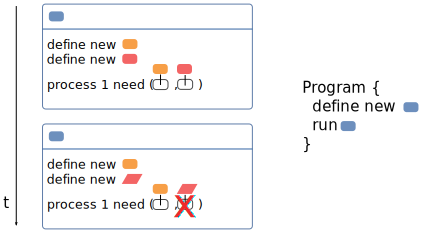
\includegraphics[width=.7\linewidth]{composants_principes_a.pdf}
  	\label{subfig_decouplage:a}}\qquad
  \subbottom[]{
	
\includegraphics[width=.8\linewidth]{composants_principes_c.pdf}
  	\label{subfig_decouplage:b}}
  \subbottom[]{
	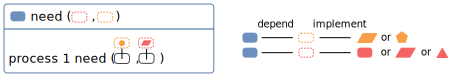
\includegraphics[width=.8\linewidth]{composants_principes_d.pdf}
  	\label{subfig_decouplage:c}}
 \end{sidecaption}
\end{figure}


Si on recontextualise ces principes à notre problèmatique, les classes de composants nécessaire à l'execution minimale d'un algorithme évolutionnaire dans MGO sont décrites dans la figure \ref{fig:cake_classe}, et s'appuie sur le travail déjà décrits de la communauté pour unifier la description des algorithmes.


\begin{figure}[!htbp]
	\begin{sidecaption}[fortoc]{Classe de composants nécessaires pour l'execution d'un EC.}[fig:cake_classe]
		\centering
		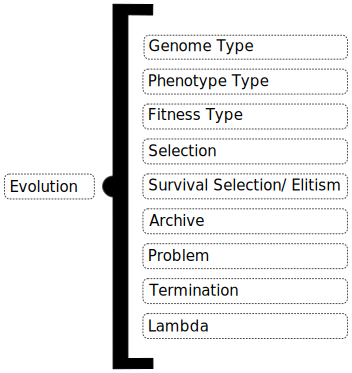
\includegraphics[width=0.7\linewidth]{cake_example.pdf}{
		}
  \end{sidecaption}
\end{figure}

Chacune de ces classes de composants est définit comme nécessaire pour le fonctionnement d'un algorithme d'évolution, dont la mise en dynamique du comportement générique est implémenté dans le composant Evolution. Tant que l'utilisateur n'aura pas fourni un composant compatible avec chacun de ces types de composants, alors le composant Evolution ne pourra pas s'executer. Le programme est définit comme un texte à trou, les boites sont bien placés, et le programme prêt à être executé suivant cet ordre, seulement ce n'est qu'un patron, une image, et cet ensemble de boite dont seule une partie de la logique à été intégré, doit encore être complété. C'est un peu comme un puzzle dans lequel il manque des pièces, vous devez soit créer de nouvelle pièces, soit retrouver les pièces qui respectent la forme de chaque trou pour que le puzzle soit de nouveau complet. 

L'inversion de controle détaillé dans les paragraphes précédents se matérialise de nouveau ici au travers du fait que c'est l'utilisateur qui définit sa composition, en s'assurant avec l'aide des instructions du programmes que les dépendances propres au fonctionnement de chacun des composants sont bien fournies. Tout programme ne remplissant pas les conditions renverra un message d'erreur à son execution. En ce sens MGO est probablement plus un \textit{framework} qu'une librairie logicielle \Anote{martin_fowler}. L'avantage d'une telle approche c'est que l'application peut être livrée avec un vaste catalogue de pièce correspondant à chaque emplacement, laissant à l'utilisateur la possibilité de choisir sa propre combinaisons, voire même de créer ses propres pièces si il estime quel sont manquantes. 

Ils existent différentes techniques pour que cette technique puisse être mise en oeuvre, mais en Scala, l'implémentation la plus courante et la plus utilisé est connu sous le nom de \foreignquote{english}{Cake Pattern}, \foreignquote{english}{Scalable Component Abstractions} ou encore \foreignquote{english}{Component Based Dependency Injection}, accessible nativement dans le langage car pensé et implémenté par son créateur Martin Odersky.

Le défaut de cette technique, c'est qu'il rend la lecture du code source plus difficile, du fait de ce morcellement dans l'appel des différentes fonctions.


\subsubsection{La mise en oeuvre du couplage MGO - openMOLE }

Le choix est fait ici de développé une librairie MGO utilisable de façon indépendante, ou de façon couplé à openMOLE. 

Les objectifs motivant la construction d'une nouvelle librairie sont les suivants : 



L'étape suivante est do nc le couplage de cette librairie avec openMOLE 


Martin Oderskys’


\begin{minted}[linenos=true,frame=single,fontsize=\footnotesize]{scala}
import fr.iscpif.mgo._
import math._
import util.Random

trait ZDT4 extends GAProblem with MGFitness {

  def min = Seq.fill(genomeSize)(0.0)
  def max = 1.0 :: Seq.fill(genomeSize - 1)(5.0)

  type P = Seq[Double]

  override def express(g: Seq[Double], rng: Random) = Seq(f1(g), f2(g))
  override def evaluate(p: P, rng: Random) = p

  def f1(x: Seq[Double]) = x(0)
  def f2(x: Seq[Double]) = g(x) * (1 - sqrt(x(0) / g(x)))
  def g(x: Seq[Double]) =
    1 + 10 * (genomeSize - 1) + (1 until genomeSize).map 
    { i => pow(x(i), 2) - 10 * cos(4 * Pi * x(i)) }.sum
}
}
\end{minted}

\section{Une brique logicielle dédiée à la visualisation de résultats}


